\documentclass[oneside, 12pt]{article}

\usepackage{amsmath}
\usepackage{amsfonts}
%\usepackage{algorithm}
%\usepackage{algorithmic}
\usepackage{multirow}
\usepackage{colortbl}
\usepackage{color}
\usepackage[table]{xcolor}
\usepackage{epigraph}
%\usepackage{subfigure}
\usepackage{caption}
\usepackage{subcaption}
\usepackage{tabularx}
\usepackage{float}
\usepackage{longtable}
\usepackage[pdftex]{graphicx}
\usepackage{pdfpages}
\usepackage{tabularx}
\usepackage{pdflscape}
\usepackage[acronym,toc]{glossaries}
\usepackage[margin=1.2in]{geometry}
\usepackage{titling}
\usepackage[T1]{fontenc}

\usepackage{listings}
\usepackage{color}

\definecolor{codegreen}{rgb}{0,0.6,0}
\definecolor{codegray}{rgb}{0.5,0.5,0.5}
\definecolor{codepurple}{rgb}{0.58,0,0.82}
\definecolor{backcolour}{rgb}{0.95,0.95,0.92}
\lstdefinestyle{mystyle}{
	backgroundcolor=\color{backcolour},   
	commentstyle=\color{codegreen},
	keywordstyle=\color{magenta},
	numberstyle=\tiny\color{codegray},
	stringstyle=\color{codepurple},
	basicstyle=\footnotesize,
	breakatwhitespace=false,         
	breaklines=true,                 
	captionpos=b,                    
	keepspaces=true,                 
	numbers=left,                    
	numbersep=5pt,                  
	showspaces=false,                
	showstringspaces=false,
	showtabs=false,                  
	tabsize=2
}

\lstdefinelanguage{JavaScript}{
	backgroundcolor=\color{backcolour},
	keywords={\$, script, for, Object, typeof, new, true, false, catch, function, return, null, catch, switch, var, if, in, while, do, else, case, break},
	keywordstyle=\color{magenta}\bfseries,
	ndkeywords={class, export, boolean, throw, implements, import, this},
	ndkeywordstyle=\color{darkgray}\bfseries,
	identifierstyle=\color{black},
	sensitive=false,
	comment=[l]{//},
	morecomment=[s]{/*}{*/},
	commentstyle=\color{codegreen},
	stringstyle=\color{codepurple},
	morestring=[b]',
	morestring=[b]"
}

\lstset{style=mystyle}

\usepackage[style=ieee,backend=biber]{biblatex}
\addbibresource{report.bib}


%\providecommand{\tightlist}{%
%	\setlength{\itemsep}{0pt}\setlength{\parskip}{0pt}}
%\setcounter{secnumdepth}{0}

\PassOptionsToPackage{hyphens}{url} % url is loaded by hyperref
\usepackage[unicode=true]{hyperref}

\setlength{\parindent}{0pt}
\setlength{\parskip}{6pt plus 2pt minus 1pt}


\pretitle{%
	\begin{center}
		\huge
		
\includegraphics[width=6cm,height=2cm]{images/reading_logo.png}\\[\bigskipamount]
	
	}
\posttitle{
	
	\large
	School of Mathematical, Physical and Computational Sciences
	\newline
	Indivdual Project - CS3IP16
\end{center}}


\title{Opinion Mining and Social Media Sentiment Analysis in the Prediction of Cryptocurrency Prices}
\date{Submission date: Place Holder}
\author{Student: Andrew Sotheran
	\\Student Number: fr005432
	\\Supervisor: Kenneth Boness
	\\Word Count: Place Holder}

\begin{document}
	
	\maketitle
	
	\vspace*{\fill}
	\begin{center}
		\section{Abstract}\label{abstract}
	\end{center}
		The volatility of the stock markets is an aspect that is both hard to predict and to mitigate particularly when relating to the cryptocurrency market. Commodities such as cryptocurrencies are profoundly volatile and have attracted investors in an attempt to make quick profits on the market. These financial commodities are subject to the whim of public confidence and platforms such as Twitter and Facebook are most notably utilised to express opinions. Extrapolating sentiment from such platforms has been used to gain insight into topics across industries, thus applying it to crypto-market analysis could serve to show a relationship between public opinion and market change. 
		
		This project looks into public perception of the cryptomarket, by analysing Bitcoin-related tweets per hour for sentiment changes that could indicate a correlation to market fluctuations in the near future. This is achieved by training a recurrent neural network on the severity changes of historical sentiment and price over the past year every hour. The predictions are then shifted forward in time by 1 hour to indicate the corresponding Bitcoin price interval.

	
	\newpage
	\begin{center}
		\section{Acknowledgements}\label{acknowledgements}
		I would like to express my gratitude to Dr. Kenneth Boness for his continued support and guidance throughout this project.  
		
		Secondly, I want to express gratitude to PhD. Jason Brownlee, of \href{machinelearningmastery.com}{Machine Learning Mastery} for having clear and thorough explanations of machine learning concepts and metrics.
		
		I would also like to thank my family for their support during the development of this project.
		
	\end{center}
	
	\newpage
	\begin{center}
		\section{Glossary}\label{glossary}
	\end{center}
	Bull(ish)/Bear(ish) Markets - Relates to a trend of the market price increasing and decreasing respectively
	
	Highs/Lows - The highest and lowest trading price of a giving period
	
	Fiat Currency - A currency without intrinsic value that has been established as money
	
	BTC - Bitcoin's stock symbol
	
	Twitter - Online social media platform, which allows users to post information or express opinions through messages called "Tweets"
	
	Tweets - The name given for messages posted on the Twitter platform, which are restricted to 280 characters.
	
	Hashtag - Is a keyword or phrase used to describe a topic and allows the tweets to be categorised.
	
	Fomo (Fear of Missing Out) - Is used to describe buying behaviour when stocks are moving suddenly and more buyers appear to enter all of a sudden.
	
	Shorting - Or short sale, is the sale of an asset that the investor buys shares and immediately sells them, hoping to make a profit from buying later at a lower price.
	
	Doubling Down - Is to take further risk on a stock by doubling effort/investment in a hope and attempt to raise the price
	
	RNN - Recurrent Neural Network - A type of neural network that remembers weights and parameters for learning
	
	LSTM - Long-Short Term Memory Neural Network - A type of recurrent neural network that overcomes limitations of standard RNNs
	
	RMSE - Root Mean Squared Error - Regression performance metric
	
	MSE - Mean Squared Error - Regression performance metric
	
	MAE - Mean Absolute Error - Regression performance metric
	
	MAPE - Mean Absolute Percentage Error - Regression performance metric
	
	HTML - Hyper-Text Markup Language - Scripting language used for forming web pages.
	
	CSS - Cascading Style Sheets - A scripting language used to customise the design of the interface of a webpage coded in HTML
	
	JSON - JavaScript Object Notation - Open Standard file format that uses human readable text to transmit data objects
	
	CSV - Comma-Separated Values - Tabular file format that uses commas to separate values
	
	API - Application Programming Interface - A set of web endpoints, communication protocols and tools for building software
	
	\newpage
	
	\begin{center}
		\tableofcontents
	\end{center}
	
	\newpage
	\begin{center}
		\section{Introduction}\label{introduction}
	\end{center}
	The premise of this project is to investigate whether the sentiment expressed in social media has a correlation to the prices of cryptocurrencies and how this could be used to predict future changes in the price. 
	
	The chosen cryptocurrency that will be of focus for this project will be the currency Bitcoin (BTC), due to having the largest community and backing and has been known to lead other fiat currencies. Bitcoin is seen as one, if not the first cryptocurrency to bring a broader following to the peer-to-peer token transaction scene since 2009. Although it was not the first token to utilise blockchain technology, it allowed investors to openly trade a public cryptocurrency which provided pseudonymous means of transferring funds through the internet. Thus it has been around longer than most of the other fiat currencies and is the most popular crypto-token due to it's more extensive community base.
	
	Most financial commodities are subject to the whim of public confidence and are the core of its base value. A platform that is frequently used for the public to convey their opinions on a commodity is that of Twitter which provides arguably biased information and opinions. Whether the opinions present a basis in facts or not, they are usually taken at face value and can influence the public opinion of given topics. As Bitcoin has been around since 2009 the opinions and information on the commodity are prevalent through the platform. 
	In the paper \textit{Sentiment Analysis of Twitter Data for Predicting Stock Market Movements} by \textit{Majhi et al.} \cite{SaTdpsmm} 2.5 million tweets on Microsoft were extracted from Twitter, sentiment analysis and logistical regression performed on the data yielded 69.01\% accuracy for a 3-day period on the increase/decrease in stock price. These results showed a "\textit{good correlation between stock market movements and the sentiments of the public expressed in Twitter}".
	
	The background of this project is in response to the volatility of the cryptocurrency market, which can fluctuate at a moments notice and can be seen to be social media driven. The history of the price of Bitcoin and what was being discussed on the currency around it's most volatile period to-date, Nov-2017 to Feb-2018, shows a strong bullish trend which saw Bitcoin reach a \$19,500 high in mid-Dec. While social media, such as Twitter, during that period was had an extremely positive outlook on the cryptocurrency. The trend was short lived and saw the market crash only a month later, with only a couple of sell-offs, expected for the holidays rush, accompanied by negative outlooks posted on social media turned the market against itself which saw the longest bearish market in Bitcoin's history and is still trying to recover today.
	
	Due to how volatile the crypto-market can be, there is a need to either mitigate or to anticipate where the markets are heading. As the crypto-market and Bitcoin are affected by socially constructed opinions, either through Twitter, news articles or other forms of media, there is a way to perform the latter, where the prices of Bitcoin could be predicted based on the sentiment gathered from social media outlets.
	
	This project aims to create a tool that gathers tweets from Twitter, obtains the overall sentiment score of the given text while gathering historical price data for the period gathering occurs. Features are then extracted from the gathered data and used in a neural network to ascertain whether the price of the currency can be predicted from the correlation between the sentiment and price history of the data.
	
	This report will discuss the justifications for the project and the problems it will be attempting to resolve, the stakeholders that would benefit the most from this system and what this project will not attempt to accomplish. Similar tools will be critiqued and examined for their feature set and credibility in the literature review along with current sentiment analysers, algorithms, natural language processing techniques and neural networks in their respective topics and comparing their accuracy for this project purpose. 
	The solution approach will discuss the decisions and reasoning behind choosing the techniques and tools used for this project and will outline the requirements for this project.
	Implementation of the chosen techniques and tools, with the discussion of essential functions of the system will formulate the implementation section of this report with an in-detail explanation of the function's use and data flow of the system.
	
	\newpage
	
	\begin{center}
		\section{Problem Articulation}\label{problem}
	\end{center}
		
		\subsection{Problem Statement}\label{statement}
		
		The fundamental problems this project attempts to address are that of, an open-source system available to the public that aids in investor decision making on whether to invest at a given point, based on the analysis and prediction of BTC for each hour. The accuracy of open-source tools and technology when applied to the trading market scene and to identify whether there is a correlation between Twitter sentiment and BTC price fluctuation. While there are existing tools, only a few are available to the public and only provide basic functionality, while others are kept in-house of major corporations who invest in this problem domain.
		
		The other issue presented here is that assuming perfect accuracy can be achieved is naive. As this project will only be using existing tools and technologies; thus, there are limitations to the accuracy of what can be obtained. One of that being the suitability of the tools, there are no open-source sentiment analysers for stock market prediction, thus finding a specifically trained analyser for the chosen domain in highly unlikely. In relation, finding the most suitable machine learning or neural network is equally important as this will determine the accuracy of the predictions. Due to being a regression problem, machine learning techniques and neural networks that focus around this and forecasting should be considered.
		
		The accuracy and suitability of various machine learning methods and neural networks are a known issue in their respective domains. This investigation should be carried out to determine their suitability for their needed use in this project and will be detailed in the literature review.
		
		This project will focus on the investigation of these technologies and tools to justify whether it is feasible to predict the price of BTC based on historical price and the sentiment gathered from Twitter. Limitations of the system and it's accuracy in predictions should be investigated and discussed to determine the implemented solution is the more suitable compared to other methods.  
		
		\subsection{Stakeholders}\label{stakeholders}
		The main stakeholders of this system would be those looking to invest in the cryptocurrency markets, in this projects regard, specifically into Bitcoin. 
		
		\begin{itemize}
			\item Public Investors - These are investors from the general public. These investors can decide to either actively or passively invest in the markets but are essential for the general use of a given cryptocurrency. This type of investor would benefit the most from an open-source system such as this, as it will aim to provide a basis for decisions for buying or selling Bitcoin. Additionally, due to the lack of any open-source tools available, these stakeholders could be seen as being left in the dark when it comes to predicting the direction of Bitcoin where Businesses and Enterprises will have a one up, due to having an internal system for predictions.
			\item Speculators - These stakeholders can be both public and business, who aim for the chance of the possibility fast. They actively invest at points where a market is an impending rise in price and tend to sell after a market makes them a reasonable amount of money before it possibly drops. These stakeholders would benefit from such a system as it will provide a means to identify and predict short term gains in the Bitcoin market, and if taken into decisions could make a profit.
			\item Business Investors: These will be investors of a business who would be investing on the behalf of a company. A system such as that this project will provide may benefit such a stakeholder, but the information would be used as a collective with others to justify the investment. Additionally, this system may not benefit this stakeholder as the company they are investing for may have an equivalent or better system.
			\item Prospect Investors: These are new investors to the cryptomarket scene who are looking to get into the market and are generally looking for initial information of the market movement. This system will benefit such a stakeholder in their initial decisions in market investment, but not as much as a generally more active investor. This is due to the extent to which a new investor invests compared to a establish active investor.
			
			\item Developer - Andrew Sotheran: The developer responsible for this project by developing a solution that satisfies the problem and	objective defined in the \textit{Technical Specification}. As the sole developer of this project it should be ensured that the system is developed on time and the project runs smoothly.
			\item Project Supervisor - Kenneth Boness: Is the projects supervisor whom will oversee the development through weekly project meetings. Weekly feedback will be given on the progress and direction of development, and will offer advice to ensure the quality of the solution.
		\end{itemize}
		
		\subsection{Project Motivation}
		The motivation behind the project stems from a range of points, from personal and public issues with the volatility if the crypto-market, and how losses specifically could be mitigated. The personal motivations behind the conceptualisation of this began two years ago during the crash of late 2017-2018, which saw new investors blindly jump into the trend that was buying cryptocurrencies. During this period of November to December 2017 saw Bitcoin's price reach \$20,000 from \$5,000, new public investors jumped on the chance to buy into the trend of possibly making quick profits and the fear of missing out (FOMO). In late December, a few holiday sell-offs occurred from business and big investors, this coupled with a few negative outlooks posted on social media by news outlets caused the market to implode causing investors to panic sell one after the other and posting negativity on social, thus causing more decline in the market. As a result, this caused personal monetary loss and distress as being a long-term investor.
		
		Another motivation is that at the time of writing, there are no publically available systems that combine sentiment analysis with a historical price to forecast the price of Bitcoin or any other cryptocurrency. There are papers and a few code repositories that implement a similar concepts \cite{nlAeiBTCPSO} - \textit{Use of a Multi-layer Perceptron network for moving averages in Bitcoin price}, \cite{BTCFTsent} - \textit{Predicting Bitcoin price fluctuation with Twitter sentiment analysis}, \cite{BTCRNN} - \textit{Predict Tomorrows Bitcoin (BTC) Price with Recurrent Neural Networks} but are not operational. A system such as \cite{SaTdpsmm} hosted on Coingecko, a popular cryptocurrency track site, provides a tool for basic sentiment analysis but doesn't give an evaluated indication of the direction of the market as a prediction. This leaves the public to the whim of volatility of the market without a means to know what the next, say an hour, could entail to possibly reduce losses if the market drops. Such systems are usually kept in-house of major corporations who invest significant time into tackling such a problem. Additionlly, this could be seen as a positive for major investors, as such a system could cause panic selling if public investors solely trusted such a system.
			
		\newpage
		\subsection{Technical Specification}
		This project will need to follow a specification to ensure that the quality and the problem statement is met. This section will outline what this project should include, what it will not consist of and will guide the development of this project.
		\newline
		
		\textbf{General}:
		\begin{itemize}
			\item To investigate into the use of lexicon-dictionary based sentiment analyser approach in for sentiment analysis and it's customisability for a given topic domain
			\item To create a system that can predict the next hour of Bitcoin's price when given the price and sentiment for the past hour
			\item To investigate into natural language data pre-processing techniques and how these could be used to filter out unwanted data
			\item To investigate into the use of a neural network, specifically an LSTM for forecasting price data
			\item Ultimatly, to investigate into how the use of sentiment effects the prediction of price for the next hour
			\newline
		\end{itemize}
		
	
		\textbf{Natural Language pre-processing (Spam and language detection filtering)}
		\begin{itemize}
			\item To produce a system that processes the historical and live tweets, removing unwanted characters, removing urls and punctuation.
			\item To produce a system for spam filter using probability likelihood for processed tweets. A naive Bayes approach may be suitable for this given task
			\item To produce a language detection and filtering system that removes all tweets that are not of the English language or containing non-basic-latin characters
			\item To provide a means for stemming, tokenisation and stopword removal to aid in data pre-processing for language detection and spam filtering
			\newline
		\end{itemize}
		
		\textbf{Neural Network}
		\begin{itemize}
			\item To produce a neural network which trains on collected, historical and live data, to forecast the future price of Bitcoin, based on price and sentiement
			\item To produce a neural netowork which accomplished the same as the other above, but with out use of sentiment
			\item To produce metrics to justify accuracy of the model
			\item To produce data files containing, the current time of predictions alongside current hour price and sentiment. This should also include a suggested action based on a threshold for the price difference between hours. 
			\item To produce data files containing the true and predicted price values of every hour for trained data, and another for current reoccuring predictions.
			\newline
		\end{itemize}
		
		\textbf{Interface}
		\begin{itemize}
			\item To produce a basic interface which displays the predicted values alongside true price values with a time interval step of an hour. This can be displayed as both a table consisting of: 
			\subitem Date of prediction, predicted price of next hour, current hour price and sentiment, and a suggested action based on a threshold for the price difference between hours.
			\subitem To produce charts displaying the true and predicted price values for every hour, from both start of new predictions made, and from training predictions
			\item To display a table of performance metrics of the trained model
			\newline
		\end{itemize}
	
		\textbf{Server}
		\begin{itemize}
			\item This system, both prediction system and interface, should be deployed to a server due to the need to be constantly running
		\end{itemize}
		
		This project will not attempt to justify the accuracy of the chosen algorithm or tools over other algorithms. It will be discussed in the solution approach the justifications made on why the chosen algorithm and tools have been used for this project over the others, but accuracy will not be directly compared.
		
		This project will only be coded to predict an hour ahead as the model will be trained on an hourly basis as the data is gathered per hour. Predictions for further in the future can be modelled but will be seen as a future improvement to the system.
		
		The detail of a interface may be subject of change through this project due to time contraints and the focus being the investigation of the impact social media has on market predictions.
	
	\newpage
	\section{Quality Goals}
	Although this project will be an investigation it is important to ensure that a specific level of quality is met and maintained throughout development to produce a final solution that fully meets the requirements set out in the technical specifiction. This section will outline the quality objectives, processes used to aid in ensuring quality, quality goals and the deveopment pipeline.
	
	\subsection{Process Description}
	To maintain a level of quality through the project's development lifecycle various processes are to be defined. As stated in ISO 9001:2015 \cite{ISO9000} "Consistent and predictable results are achieved more effectively and efficiently when activities are understood and managed as interrelated processes". To achieve this, clearly defined processes of how this system should be developed along with tools to achieve this will need to be defined before the development of this project, to ensure an effective, transparent and well-tested system is created, of which should be outlined in the solution approach.
	
	\subsection{Quality Objectives}
	The objective of testing is to determine that the functionality provided works according to the specifications and satisfies the problem statement. This is to ensure that the system is performing both as intended and without failure.
	
	The most important aspect of testing of the system is to ensure that predictions for Bitcoin price are calculated for the next hour interval. Testing should be conducted around this to both determine the accuracy of the predictions made by the system, and to validate the optimisers and other methods used for model creation. Suitable performance and accuracy metrics should be chosen and implemented to aid in justifying the accuracy of the developed solution for a regression model.
	
	The development of this project should follow an agile methodology as closely as and when possible. Prior to functions and components being created after another has finished development, said completed function should be tested and fully operational with the existing functions and components it uses or provides for. Integration testing should be conducted to determine what functions are operating as intended along with the development of the system.
	
	Lastly, the testing of the user interface shouldn't be considered as part of the testing of the system due to the focus of this project not formulating around the development of the interface, but rather around the back-end prediction system. As long as what is intended to be displayed to the user and are displayed correctly as per the user interface design such testing will be sufficient.
	
	\subsection{Tools to Ensure Quality}
	
	\begin{itemize}
		\item Version Control: A version control system will be used for the development of this project, such as Git - (Github), and will provide a means to track the versions of the code and to store it on a remote server as a backup.
		\item Linting and Static code analysis: This will allow for an on-the-fly bug detection and code quality measures to be set for the python language. This will ensure that code is written in the best practice for the language and all code will conform to the same standard. The type of linting analyser that will be used will be determined by the Text editor used for development.
		\item Text Editor/IDE: Visual Studio Editor will be used as the sole text editor for the development of this project, due to having an in-built python linter.
	\end{itemize}
	
	\newpage
	
	\begin{center}
		\section{Literature Review}\label{literature}
	\end{center}
		\subsection{Existing Tools}
		An aspect that this project will be attempting to address is that, at the time of writing, there are a limited amount of systems available to the public that either provide sentiment analysis or predictions of the crypto-market. Additionally, none known that combine both sentiment and price analysis to make said predictions on the direction of the market.
		
		Such tools are usually provided by exchanges which correspond the amount of positive and negative sentiments with a suggestion to buy and sell. These tools, however, are vague in their suggestions as they don't provide any further analysis on when the best time would be to conduct an action on the market, and simply display the number of tweets per sentiment level. A well-known cryptocurrency tracking site,\href{https://www.coingecko.com}{Coingecko} provides a basic sentiment analysis tool for their top 30 ranking cryptocurrencies tracked on the site. This tool shows the sentiment analysis of tweets from Twitter every hour for a given cryptocurrency. This is displayed as a simple pill on the page showing the ratios of positive, neutral and negative tweets. \textit{See Appendix C for visual representation}
			
		\subsection{Related research}
		
		There has been an abundant amount of research conducted in this problem domain. Many theses globally have been published in recent years on the topic of cryptocurrency market predictions and analysis, and even more, research conducted on general stock markets further back. 
		
		The thesis written by \textit{Evita Stenqvist and Jacob Lonno} of the \textit{KTH Royal Institute of Technology} \cite{BTCFTsent} investigates the use of sentiment expressed through micro-blogging such as Twitter can have on the price fluctuations of Bitcoin. Its primary focus was creating an analyser for the sentiment of tweets more accurately \textit{"by not only taking into account negation, but also valence, common slang and smileys"}, than that of former researchers that \textit{"mused that accounting for negations in text may be a step in the direction of more accurate predictions."}. This would be built upon the lexicon-based sentiment analyser VADER to ascertain the overall sentiment scores were grouped into time-series for each interval from 5 minutes to 4 hours, along with the interval prices for Bitcoin. The model chosen was a naive binary classified vectors of predictions for a certain threshold to \textit{"ultimately compare the predictions to actual historical price data"}. The results of this research suggest that a binary classification model of varying threshold over time-shifts in time-series data was "lackluster", seeing the number of predictions decreasing rapidly as the threshold changed. This research is a reasonable basis of starting research upon, as it suggests tools such as VADER for sentiment analysis and that the use of a machine learning algorithm would be a next step in the project that would yield better more accurate results.
		
		Another thesis written by \textit{Pagolu, Venkata Sasank and Reddy Kamal Nayan, Panda Ganapati and Majhi, Babita} \cite{SaTdpsmm} on "Sentiment Analysis of Twitter Data for Predicting Stock Market Movements" 2.5 million tweets on Microsoft were extracted from Twitter, sentiment analysis and logistical regression performed on the data yielded 69.01\% accuracy for a 3-day period on the increase/decrease in stock price. These results showed a "\textit{good correlation between stock market movements and the sentiments of the public expressed in Twitter}". Using various natural language pre-processing tweets for feature extraction such as N-gram representation the sentiment from tweets were extrapolated. Both Word2vec and a random forest classifier were compared for accuracy, Word2vec being chosen over the machine learning model. Word2vec, being a group of related shallow two-layer neural network models to produce word embeddings.
		
		A topic that reoccurs in various papers and theses is that of the use and focus of regression techniques and machine learning methods. Few implement a fully fledged neural network; the above paper attempts to use a simple network to achieve predictions of classification of sentiment for stock market movement then correlated this with historical data of prices. An article posted on "Code Project" by Intel Corporation \cite{StPNSentA} compares the accuracy of three machine learning algorithms; Random Forest, Logistic Regression and Multi-Layer Perceptron (MLP) classifiers on predicting the price fluctuations of Bitcoin with embedded price indices. Results showing \textit{"that using the MLP classifier (a.k.a. neural networks) showed better results than logistic regression and random forest trained models"}. This assumption can be backed up by the results from a thesis posted on IEEE \cite{MLBTCpred} which compares a Bayesian optimised recurrent neural network and a Long Short Term Memory (LSTM) network - showing the LSTM model achieving \textit{"the highest classification accuracy of 52\% and a RMSE of 8\%"}. With interest in neural networks personally and with little papers utilising them for this purpose a neural network will thus be implemented, and the accuracy of one's predictions with use of sentiment analysis data analysed and discussed.
			
		\subsection{Data Collection}\label{tweet_collection}
			
			\subsubsection{Twitter and Twitter API}
			Twitter is a micro-blogging platform that was launched in 2006 and provides it's users the ability to publish short messages of 140 characters. The messages published could be of any form, from news snippets, advertisement, or the prevalent publication of opinions which allowed a platform of extensive diversity and knowledge wealth. As of the time of writing, the message character limit was increased to 280 characters, the platform has over 300 million monthly active users, and around 1 million tweets are published per day. Due to the length restriction and the primary use of the platform to express opinions Twitter is seen as a gold mine for opinion mining.
			
			The Twitter API has an extensive range of endpoints that provide access from streaming tweets for a given hashtag, obtaining historical tweets for a given time-period and hashtag, posting tweets on a users account and to change settings on a user account with authentication. The exhaustive range of features provided by these endpoints makes data collection from Twitter straight forward as one can target a specific endpoint for the required data. Due to Twitter being the target for opinion mining within this project the Twitter API will ultimately need to be utilised. This can either be used for the gathering of historical tweets or streaming current tweets for the \#Bitcoin hashtag.
			
			There are, however, limitations and rate limits imposed on users of the API. Twitter employs a tiering system for the API - Standard, Premium and Enterprise tiers, each of which provides different amounts of access for data collection. If the API were to be used to capture historical data for a span of 3 months, each tier is allowed to obtain varying amounts of data for different durations; \cite{SearchTweets}
			
			\begin{itemize}
				\item A Standard user would be able to capture 100 recent tweets for the past 7 days
				\item A Premium user would be allowed to capture up to 500 tweets per request for a 30-day span and will have access to a full-archive search to query up to 100 tweets per request for a given time period, with a 50 request limit per month
				\item An Enterprise user would be able to capture up to 500 tweets per unlimited requests for a 30-day span and will be able to query the full-archive of tweets for a given hashtag up to 2000 tweets per unlimited amount of requests for a given time period
			\end{itemize}
		
			Each tier has individual costs while the standard user negating this as a basic tier. Due to only being elegable for the Premium tier for educational purposes, historical data gathering will be limited to 100 tweets per request with a limitation of 50 requests per month. Furthermore streaming tweets is an Enterprise feature which rules out the the Twitter API for use of streaming current real-time data \cite{ConStream}.
		
			\subsubsection{Tweepy Python Package}
			Tweepy is a python package for accessing the Twitter API. It fundamentally accomplishes the same means if one to conduct a GET request to the Twitter API, except it simplifies this into a simple to use API that is easier to implement and automate in python \cite{TweepyStream}. Consequently, it builds upon the existing Twitter API to provide features such as automated streaming of provided hashtags to the API. It realises this by initialising a listener instance for a provided set of API credentials, handling authentication, connections, creating and destroying sessions. Due to Twitter's streaming API being only available to Enterprise users \cite{SearchTweets}, using Tweepy to stream data for a given hashtag will provide the real-time data needed. The streaming of current data by Tweepy is accomplished by setting up a stream which listens for new data for a given hashtag, which bypasses the need for the Enterprise tweet tracker provided by the Twitter API.
			
		
		\subsection{Sentiment Analysis}\label{sentiment}
		In short, sentiment analysis is the process and discovery of computationally identifying and categorising the underlining opinions and subjectivity expressed in written language. This process determines the writer's attitude towards a particular topic as either being positive, neutral or negative in terms of opinion, known as polarity classification. 		
			
			\subsubsection{Natural Language Processing}\label{algorithms}
			Polarity classification is the focus of sentiment analysis and is a well-known problem in natural language processing that has had significant attention by researchers in recent years \cite{SaTdpsmm}\cite{BTCFTsent}\cite{MLBTCpred}\cite{PolClassPatients}. Traditional approaches to this have usually been classified to dictionary-based approaches that use pre-constructed sentiment lexicons such as VADER or usually confined to machine learning approaches. The latter requires an extensive amount of natural language pre-processing to extrapolate vectors and features from the given text; this is then fed into a machine learning classifier which attempts to categorise words to a level of sentiment polarity. Natural language pre-processing techniques, supported by the NLTK (Natural Language Toolkit) python package that would be required for this approach would consist of;
			
			\begin{itemize}
				\item Tokenisation: The act of splitting a stream of text into smaller units of typographical tokens which isolate unneeded punctuation.
				\item Removal of domain specific expressions that are not part of general purpose English tokenisers - a particular problem with the nature of the language used in tweets, with @-mentions and \#-hashtags
				\item Stopword removal: Are commonly used words (such as "the","in","a") that provide no meaning to the sentiment of a given text
				\item Stemming: Is used to replace words with common suffixes and prefixes, as in "go" and "goes" fundamentally convey the same meaning. A stemmer will replace such words with their reduced counterparts
				\item Term Probability Identification and Feature Extraction: This is a process that involves identifying the most frequently used words in a given text, by using a probability type approach on a pre-defined dataset which classifies a range of texts as with overall negative or positive a machine learning algorithm is trained to classify these accordingly.
				\item Ngrams: Are a contiguous sequence of n items from a given sample of text. The use of Ngrams in natural language processing can improve the accuracy of classification. For example: 'Good' and 'Not Good' have opposite meanings. By only using 1 token (1gram) 'not good' ('not' and 'good') can be incorrectly classified. As the english language contains a significant amount of 2gram type word chains using 2gram can improve the accuracy of classification.
			\end{itemize}
			
			The former, seen and has been proven to provide higher accuracy than traditional machine learning approaches \cite{LexiconSocSent}, and need little pre-processing conducted on the data as words have a pre-defined sentiment classification in a provided lexicon. Although these lexicons can be complex to create, they generally require little resources to use and alter.
			
			\subsubsection{Valence Aware Dictionary and sEntiment Reasoning}\label{Vader}
				VADER is a combined lexicon and rule-based sentiment analysis tool that is specifically attuned to sentiments expressed in social media and works well on texts from other domains. It is capable of detecting the polarity of a given text - positivity, neutrality, and negativity \cite{VADERPaper}, and also calculate the compound score which is calculated by summing the valence scores of each word in the lexicon. VADER uses a human-centric approach to sentiment analysis, combining qualitative analysis and empirical validation by using human raters to rate the level of sentiment for words in its lexicon. Vader also has emoticon support which maps these colloquialisms have pre-defined intensities in its lexicon, which makes VADER specifically suitable for the social media domain were the use of emoticons, utf-8 emojis and slang such as "Lol" and "Yolo" are prevalent within the text. Additionally, VADER is provided as a lexicon and a python library under the MIT license, this means that it is open-source software. This means that the lexicon can be altered and added to abling it to be tailored to specific topic domains. 
				
				VADER was constructed by examining and extracting features from three pre-existing well-established and human-validated sentiment lexicons \cite{VADERPaper} - (LIWC) Linguistic Inquiry and Word Count, (ANEW) Affective Norms for English Words, and (GI) General Inquirer. This is supplemented with additional lexicon features \textit{"commonly used to express sentiment in social media text (emoticons, acronyms and slang)"} \cite{VADERPaper} and uses "wisdom-of-the-crowd" approach \cite{WisCrowds} to establish a point of estimations of sentiment valance for each lexical feature candidate. This was evaluated for the impact of grammatical and syntactical rules and 7,500+ lexical features, with mean valence \textit{"<> zero, and SD <= 2.5"} as a human-validated "gold-standard" sentiment lexicon. \cite{VADERPaper}\textit{Section 3.1}
				
				VADER is seen as a "Gold Standard" for sentiment analysis, in the paper for VADER, \cite{VADERPaper} \textit{A Parsimonious Rule-based Model for Sentiment Analysis of Social Media Text}, it was compared against 11 other \textit{"highly regarded sentiment analysis tools/techniques on a corpus of over 4.2K tweets"} for polarity classification across 4 domains. Results showing VADER, across Social media text, Amazon reviews, movie reviews and Newspaper editorials, consistently outperforming other sentiment analysis tools and techniques showing a particular trend in performing significantly higher on analysis of sentiment in tweets. \cite{VADERPaper} \textit{Section 4: Results}
			
		\subsection{Neural Networks}\label{networks}
			A neural network is a set of perceptrons modelled loosely after the human brain that is designed to recognise patterns in whatever domain it is intended to be trained using. A neural network can consist of multiple machine perceptrons or clustering layers in a large mesh network, and the patterns they recognise are numerical which are contained in vectors. Pre-processed data, confined and processed into pre-defined vector labels, are used to teach a neural network for a given task. While this differs from how an algorithm is coded to a particular task, neural networks cannot be programmed directly for the task. The requirement is for them to learn from the information by use of different learning strategies; \cite{NNDLBegin}\cite{WhatNN}
			
			\begin{center}
				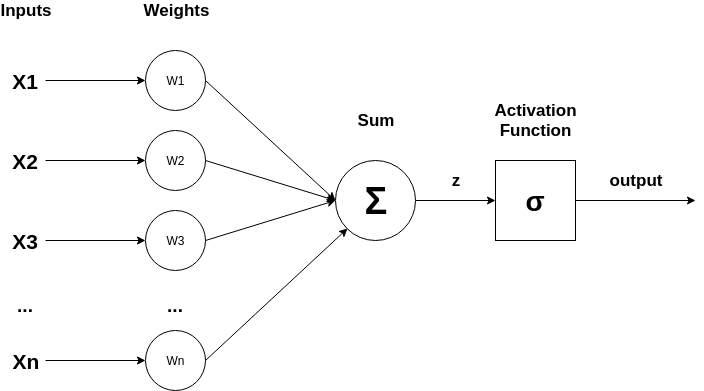
\includegraphics[width=10cm,height=6cm]{images/perceptron.png}
				\newline
				\textit{Figure 1: Basic perceptron layout}
			\end{center}
			
			\begin{itemize}
				\item Supervised learning: Simplest of the learning forms, where a dataset have been labeled which indicate the correct classified data. The input data is learned upon until the desired result of the label is reached \cite{SupdictL}
				\item Unsupervised learning: Is training the with a dataset without labels to learn from. The neural network analyses the dataset with a cost function which tells the neural network how far off target a prediction was. The neural network then adjusts input weights in attempt to increase accuracy. \cite{WhatNN}
				\item Reinforced learning: The neural network is reinforced with positive results and punished for negative results causing a network to learn over iterations. 
			\end{itemize}
		
			\subsubsection{Recurrent Neural Network (RNN)}\label{types}
			The type of neural network that is of focus for this project will be that of a Long-Short Term Memory (LSTM); however, it is crucial to understand how this is an extension of a Recurrent Neural Network (RNN) and how the underlying network works.
			
			Recurrent Neural Networks (RNN) are a robust and powerful type of neural network and is considered to be among the most encouraging algorithms for the use of classification, due to the fact of having internal memory. RNNs are designed to recognise patterns in sequences of presented data or most suitably, time-series data, genomes, handwriting and stock market data. Although RNNs were conceptualised and invented back in the 1980s \cite{ErrorProp}, they've only really shown their potential in recent years, with the increase of computational power due to the level of sequencing and internal memory store to retrain.
			Due to this 'internal' memory loop, RNNs are able to remember data and adjust neurons based on failures and alternating parameters. The way this is accomplished, knowing how a standard neural network such as a feed-forward network, should initially be understood. \cite{BeginLSTMRNN}
			
			A standard, feed-forward neural network has a single data flow with an input layer, through hidden computational layers, to an output layer. Therefore any node in the network will never see the same data again. However, in an RNN data is cycled through a loop over the same node, thus two inputs into the perception. Decisions are influenced by previous data that it has previously learned from if any, which in turn affects output and the weights of the network. \cite{RNNLSTMtds}
			
			\begin{center}
				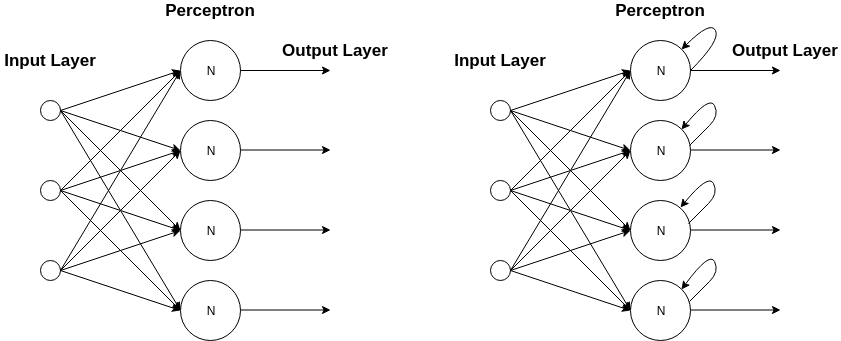
\includegraphics[width=15cm,height=6cm]{images/rnn_ffn.png}
				\newline
				\textit{Figure 2: Feed-forward network (left) vs Recurrent Neural network (right)}
			\end{center}
		
			The act of tweaking weights to alter the processing of the next iteration of data in an RNN is called backpropagation, which in short means going back through the network to find the partial derivatives of the error with respect to the weights after output has occurred. Along with gradient descent, an algorithm that adjusts the weights up or down depending on which would reduce the error. There are however a few obstacles of RNNs;
			
			\begin{itemize}
				\item Exploding Gradients: Is when gradient decsent assigns high importance to the weights. As in the algorithm assigns a ridiculously high or low value for the weights on iteration which can cause overlow and result in NaN values \cite{NNEgrad}
				\item Vanishing Gradients: Is when the values of a gradient are small enough that weights cannot be altered and the model stops learning. \cite{RNNvanishGrad}
			\end{itemize}
		
			These issues are overcome by the concept of Long-Short Term Memory neural networks, coined by \textit{Sepp Hochreiter and Juergen Schmidhuber, 1997} \cite{LSTM}. 
			
			\subsubsection{Long-Short Term Memory (LSTM)}\label{lstms}
			LSTMs are an extension of recurrent neural networks capable of learning long-term dependancies and were conceptualised by \textit{Sepp Hochreiter and Juergen Schmidhuber, 1997} \cite{LSTM}. LSTMs were explicity designed to avoid long-term dependancy problems such as exploding and vanishing gradients. As they are an extension of RNNs they operating in almost the exact same manner, but stores the actual gradients and weights in memory which allows for LSTMs to read, write and alter the values. A way of explaining how this works is seeing the memory block as a gated cell, where 'gated' is that the cell decides whether or not to store or alter data in it's memory based input data and the importance assigned to it. In a sense it learns over time of which values and data is important.
			
			\begin{center}
				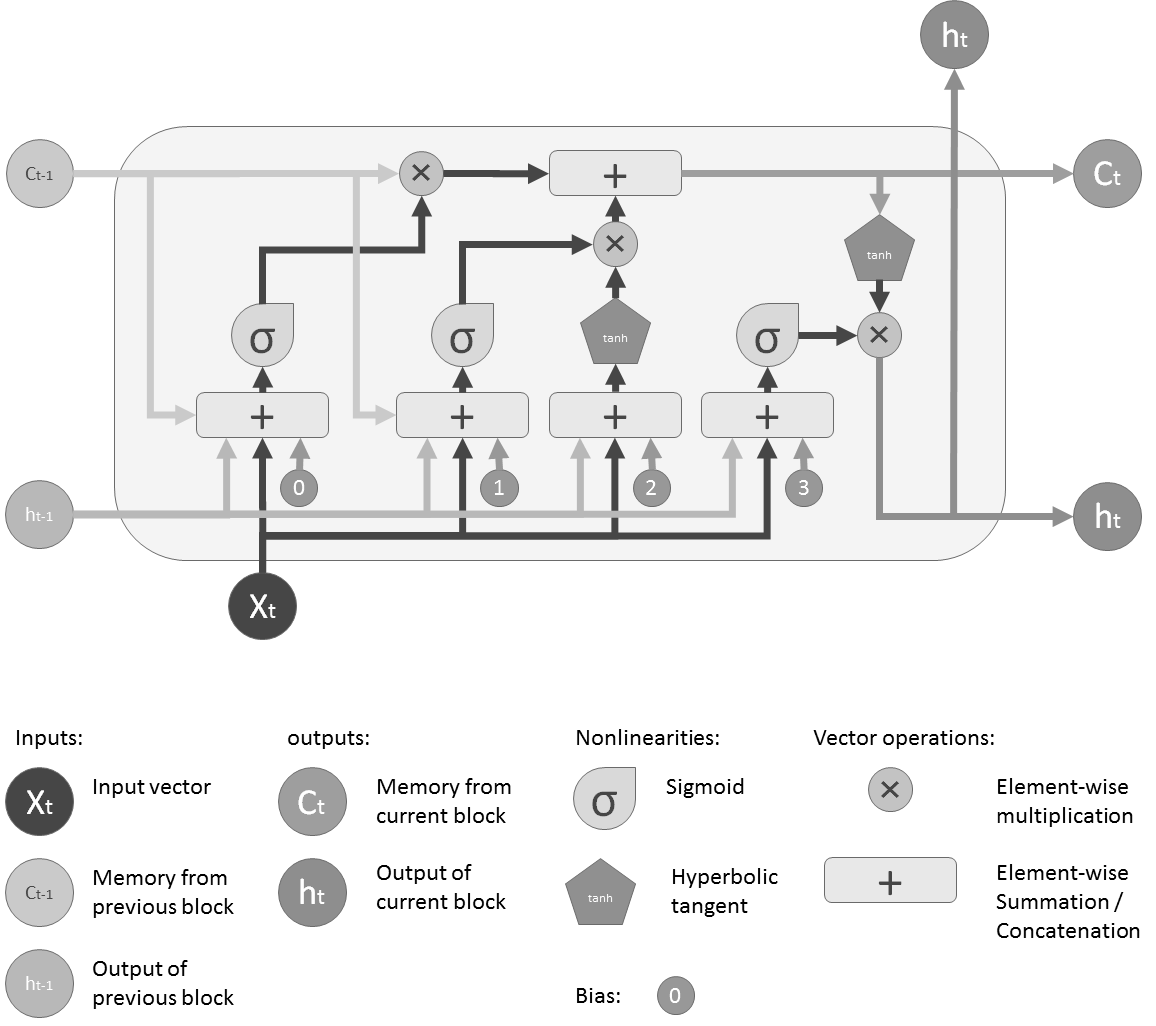
\includegraphics[width=9cm,height=7cm]{images/lstm.png}
				\newline
				\textit{Figure 3: A conceptual design of an LSTM cell bank - from Medium article by Shi Yan: Understanding LSTM and its diagrams}\cite{LSTMdia}
			\end{center}
			
			The network takes in three initial inputs, the input of the current time step, output from the previous LSTM unit if any, and the memory of the previous unit. Outputs, $H_t$ - output of current network, and $C_t$ - the memory of the current unit. \cite{LSTMdia}
			
			The various steps of the network decide what information is thrown away from the cell state, through use of a 'forget gate' which is influenced by the calculations of sigmoid memory gates which influence how much of old and new memory is used $C_{t_-1}$, $H_{t-1}$
			and $X_t$, and merged based upon importance. The section of the cell that controls the outflow memory $H_t$ and $C_t$ determines how much of the new memory should be used by the next LSTM unit. 
			\textit{For a more in-detailed explanation of exactly how the calculations are made see} \cite{LSTM},\cite{LSTMdia} and \cite{LSTMmaths}.
			
			As mentioned in the foremost section of related work the use of an LSTM network would be optimal for the given problem domain over the use of machine learning algorithms, for time-series data. As detailed above, LSTMs are widely used for time-series data forecasting due to being able to remember previous data and weights over long sequence spans\cite{LSTM}\cite{LSTMforetime}. The flexibility of LSTMs such as many-to-many models, useful \textit{"to predict multiple future time steps at once given all the previous inputs"} due to use of look-back windows and control of multiple 3D input parameters.\cite{LSTMforetime}
			
			\subsubsection{Keras and TensorFlow}
			TensorFlow is an open-source numerical math computational library framework for dataflow differentiable programming, primarily used for machine and deep learning applications such as neural networks. TensorFlow bundles various machine learning and deep learning models and algorithms into one package for the Python language, but executes as byte code executed in C++ for performance. TensorFlow provides a range of conveniences to developers for the types of algorithms it supports such as debugging models and modifying graph operations separately instead of constructing and evaluating all at once, and compatibility to execute on CPUs or GPUs \cite{TensorFlow}. However, TensorFlow's implementation and API, although provides an abstraction for development for machine and deep learning algorithms and simplifies implementation, it isn't all too friendly to programmers to use, especially new developers to the field of machine and deep learning.
			
			Keras is a high-level built to run atop of deep learning libraries such as Tensorflow and Theanos - another deep learning library similar to Tensorflow. It is designed to further simplify the use and application of such deep learning libraries thus making implementing a neural network and similar supported algorithms friendlier to developers working in Python. It accomplishes this by being a modular API; neural layers, cost functions, optimisers, activation functions, and regularisation schemes are all standalone features of the API that can be combined to create functional or sequential models. Due to being a high-level API for a more refined and more natural development of deep learning libraries, it does not provide these low-level operations and algorithms; Keras relies on a back-end engine such as TensorFlow and supports a wide range of others.
			
			\subsubsection{Optimisers}
			There are three distinct optimisers used for LSTM networks; ADAgrad optimizer, RMSprop, Adam. The role of an optimiser
			All three of which is a type of Stochastic Gradient Descent, which $\theta$ (weights of LSTM) is changed according to the gradient of the loss with respect to $\theta$. Where $\alpha$ is the learning rate and $L$ is the gradient loss. \cite{OptSGD}
			
			\[\theta_{t+1} = \theta_t - \alpha \delta L(\theta_t)\]
			
			This is primarily used in recurrent LSTM neural networks to adjust weights up or down depending on which would reduce the error, \textit{see RNN section for non LSTM limitations}. The concept of using momentum $\mu$ in stochastic gradient decent helps to negate significant convergance and divergance during calculation of the weights and dampens the oscillation, by increasing the speed of the learning rate upon each iteration. \cite{Optimisers}
			
			\[\theta_{t+1} = \theta_t + v_{t+1} \] 
			\begin{center}
				where
			\end{center} 
			\[v_{t+1} = \mu v_t - \alpha \delta L(\theta_t)\]\cite{Optimisers}		
			
			\begin{itemize}
				\item Adagrad (Adaptive Gradient): Is a method for adaptive rate learning through adaptively changing the learning parameters. This involves performing more substantial updates for infrequent parameters and smaller updates for frequent parameters. This algorithm fundamentally eliminates the need to tune the learning rate of the neural network manually and is well suited with sparse data in a large scale network. \cite{Optimisers}
				\[\theta_{t+1} = \theta_t + v_{t+1} \frac{\eta}{\sqrt{G_t + \epsilon}} \cdot g_t\]
				\begin{center}
					($G_t$ is the sum of the squares of the past gradients to $\theta$)
				\end{center}
				
				\item RMSProp (Root Mean Square Propagation): Aims to resolve Adagrad's radically diminishing learning rates by using a moving average of the squared gradient. Thus utilises the magnitude of the recent gradient descent to normalise it, and gets adjusted automatically by choosing different learning rate for each parameter. \cite{OptVariants}
				
				\[\theta_{t+1} = \theta_t - \frac{\eta}{\sqrt{(1 - \gamma) g^2_{t-1} + \gamma g_t + \epsilon}} \cdot g_t\]
				
				\begin{center}
					($\gamma$ - decay that takes value from 0-1. $g_t$ - moving average of squared gradients)
				\end{center} \cite{OverOpt}
				
				\item Adam (Adaptive Moment Estimation): Also aims to resolve Adagrad's diminishing learning rates, by calculates the adaptive learning rate for each parameter. Being one of the most popular gradient descent optimisation algorithms, it estimates from the 1st and 2nd moments of gradients. Adam implements the exponential moving average of the gradients to scale the learning rate of the network and keeps an average of past gradients. \cite{Adam}
				
				\[m_t = \beta_1 m_{t-1} + (1 - \beta_1) g_t\]
				\[v_t = \beta_2 v_{t-1} + (1 - \beta_2) g^2_t\]
				
				The algorithm updates the moving averages of the gradient ($m_t$) and the squared gradient ($v_t$) which are the estimates of the 1st and 2nd moments respectively. The hyperparameters $\beta_1$ and $\beta_2$ control the decay rates of the moving averages. These are initialised as 0 as a biased estimations for the initial timesteps, but an become bias-corrected by counteracting them with;
				
				\[ \vec{m}_t = \frac{m_t}{1 - \beta^t_1} \] 
				\begin{center}
					and
				\end{center}				
				\[\vec{v}_t = \frac{v_t}{1 - \beta^t_2} \]
				
				Thus the final formula for the Adam optimiser is;
				
				\[\theta_{t+1} = \theta_t - \frac{\eta \vec{m}_t}{\sqrt{\vec{v}_t + \epsilon}} \]
				
				\begin{center}
					\textit{Diederik P. Kingma, Jimmy Lei Ba - Adam: A method for Stochastic Optimization}\cite{Adam}
				\end{center}
			\end{itemize}
		
		\subsubsection{Regularisation}
		To avoid issues such as overfitting of the model of a neural network, techniques such as regularisation to produce better predictive performance and to improve variance of the model created. \cite{RegularisationSc} Regularisation is a technique that involves modifying the error function of the network, calculated as the sum of squares errors for individual training and validation samples. This adds a term to the error function which decreases the weights and biases of the network to smooth out outputs of each layer and LSTM cell, thus making the network less likely to overfit. 
		
		\subsubsection{Dropout}
		Dropout is a method of reducing under and overfitting of a network, by ignoring neurons during the training phase of model creation where a particular set of neurons are chosen at random to be ignored. Due to connected layers in a neural network, especially in an LSTM network, occupy the majority of the parameters neurons can develop a co-dependency on and from each other during the training phase of the network which reduces the individual efficiency of each neuron and can lead to the overfitting of training data. \cite{dropoutKeras}\cite{dropoutM}
		
		\subsection{Machine Learning}\label{machine}
			\subsubsection{Naive Bayes}
			To get an understanding of both how probability works and how a neural network will predict the next hour value based on the concepts of probability, using a well-established probability algorithm will aid in this understanding.
			
			Bayes theorem works on conditional probability and is the probability of how often an event will happen given that that event has already occurred. There are numerous variations of the theorem such as Multinomial, which supports categorical features where each conforms to a multinomial distribution, and Gaussian naive Bayes, which support continuous-valued features each of which conforming to a Gaussian (normal) distribution. The classical multinomial Bayes theorem is defined as; \cite{StudyNBC}
			
			\[P(H\cap A) = \frac{P(A\cap H) * P(H)}{P(A)} \] 
			
			\begin{center}
				and incase H and A are independant
			\end{center}
		
			\[P(H\cap A) = P(H) => P(H\cap A) = P(H)P(A)\]
			
			where:
			\begin{itemize}
				\item $P(H)$ is the probability of hypothesis being true
				\item $P(A)$ is the probability of evidence
				\item $P(A\cap H)$ is the probability of the evidence such that the hypothesis is true
				\item $P(H\cap A)$ is the probability of the hypothesis given the occurance of evidence of the probability
			\end{itemize}
		
			The naive approach assumes the features that are used in the model are independent of one another, such that, changing the value of a feature doesn't directly influence the value of the other features used in the model. When such features are independent, the Bayes algorithm can be expanded:
			
			\[P(H\cap A) = \frac{P(A\cap H) * P(H)}{P(A)} \]
			
			\begin{center}
				Becomes
			\end{center}
			
			\[P(H\cap A_1 ... A_n) = \frac{P(A_1\cap H) * P(A_2\cap H) ... * P(A_n\cap H) * P(H)}{P(A_1) * P(A_2) ... * P(A_n)} \]
			
			\[Probability \ of \ Outcome\ \cap \ Evidence = \frac{Probability \ of \ Likelihood \ of \ evidence * Prior}{Probability \ of \ Evidence} \]
			
			The naive Bayes approach has many applications, especially for the topic of this project in classifying the probability occurrence of the next price. Although it is a robust algorithm has its drawbacks which make it not as suitable as a neural network for the given need of this project. The naive Bayes trap is an issue that may occur due to the size of the dataset that will be used. There are however other scenarios this algorithm could be used such as classification of spam data.\cite{StudyNBC}
			
			\subsection{Bag Of Words}
			The Bag Of Words algorithm counts the occurance ('Term-Frequency') of a word in a given text or document. The counts allow the comparison for text classification and is used prior to TF-IDF (detailed below) to aid in identifying the probability of words in a given text and classify accordingly. \cite{TFIDFBOW}
			
			\[P(w) \ and\ P(w|spam) = \frac{Total\ number\ of\ occurrences\ of\ w\ in\ dataset}{Total\ number\ of\ words\ in\ dataset}\]
			
			\subsection{TF-IDF}
			Stands for Term Frequency-Inverse Document Frequency is another way similar to Bag of Words that are used to judge the topic of a given text. Each word is given a weight (relevance not frequency) for how many times it occurs in the given text \cite{TFIDFBOW}. 
			Term-frequency measures the number of times that a word appears in the text, but due to words such as 'and', 'the' and 'a' can frequently appear in text Inverse Document Frequency is used to change the weight of words that appear the most. Therefore words that appear the most are signalled to be less important and valuable, and therefore will not be used for classifications when used with such models as Naive Bayes for a given purpose. \cite{TFIDFBOW}
			\newline
			
			IDF is defined as:
			
			\[IDF(w) = log\frac{Total\ number\ of\ messages}{Total\ number\ of\ messages\ containing\ w}\]
			
			TF-IDF is thus defined as both:
			
			\[P(w) = \frac{TF(w)*IDF(w)}{\sum _{a\ words\ x\ \epsilon\ train\ dataset} TF(x)*IDF(x)}\]
			
			\[P(w|spam) = \frac{TF(w)*IDF(w)}{\sum _{a\ words\ x\ \epsilon\ train\ dataset} TF(x|spam)*IDF(x)}\]
				
			\cite{SpamCScratch}
			
			\subsection{Addictive Smoothing}
			Used alongside Bag Of Words, is a method of handling data that is in the test data but not in the training dataset. In case of $P(w)$ it would evaluate to 0, which will make the $P(w|spam)$ undefined as it will not be able to classify the word. Addictive smoothing tackles this by adding a number $\alpha$ to the numerator, and adding $alpha$ time the number of classes over the probability that is found in the denominator. \cite{SpamCScratch}
			\newline
			
			For TF-IDF:
			
			\[P(w|spam) = \frac{TF(w)*IDF(w) + \alpha}{\sum _{a\ words\ x\ \epsilon\ train\ dataset} TF(x|spam)*IDF(x) + \alpha\sum_{a\ words\ x\ \epsilon\ train\ dataset}}\]
			
			\subsection{Regression Performance Metrics}
			Due to the problem statement and concept behind this project is that of a regression method, forecasting and predicting a future value, performance and accuracy of such a model will ultimatly need to be identified.
			
			\begin{itemize}
				\item RMSE - Root Mean Squared Error: Represents the sample standard deviation of difference between predicted values and observed values, known as residuals. It identifies how concentrated the data is around the line of best fit, lower the better. \cite{RMSEMAE}
				\item MSE - Mean Squared Error: Is the average squared difference between the estimated values. \textit{"MSE is a risk function, corresponding to the expected value of the squared error loss."} \cite{MSE}.
				\item MAE - Mean Absolute Error: Is the average of the absolute difference between the predicted values and observed values, and is a linear score. This means that the idividual differences are weighted equally in the average. \cite{RMSEMAE}
				\item MAPE - Mean Absolute Percentage Error: Is a measure of how accuracte a forecast system is, it measures the accuracy as a percentage error for each time period minus the actual valuse divided by the actual values. \cite{MAPE}
			\end{itemize}
		
	\newpage
	
	\begin{center}
		\section{Solution Approach}\label{solution}
	\end{center}
		This section will outline the solution intended to solve the problem that the problem statement identifies, with justification and reference to the research conducted in the literature review. This will lay out the development process for the project and will tools and technologies will be explained for the particular use case in this project.
		\newline
		
		\subsection{Data gathering}
		This will be the part of the system that will gather price data and tweets from relevant sources, Twitter and cryptocurrency exchanges.
		\newline
		
		\textbf{Price data}
		\newline
		\newline
		Historical price data can be collected in a number methods, one being that of the exchange APIs, another through a historical price tracker who creates a CSV consisting of all prior historical data. Both have their merits and reliability for granting the needed data; however, a historical tracker who has been tracking the price every hour since the start of Bitcoin would be the better option. This is due to a couple of factors, the data in some historical trackers are an average unbiased price for Bitcoin - they track the price of all or a select few exchanges and average the hourly price. Whereas if the historical data was obtained directly from an exchange this would be biased and might not represent the true price of the currency, and thus would need averaging with other hourly prices from other exchanges. By using a historical tracker, all the data is unbiased and averaged and readily available and doesn't require any requests to an API or coding needed to process data.
		
		Live price data can be collected through the same methods, a historical price tracker and an exchange API. However, this doesn't work the same way; unfortunately, a historical price tracker is not updated as frequently as exchange APIs thus wouldn't provide on the hour accurate data. Therefore exchange APIs will be utilised in this case and multiple to give an unbiased average for the hourly price. Three exchanges will provide a sufficient average, and the exchanges most likely to be used would be the more popular exchanges such as Coinbase, Bitfinex and Gemini.
		\newline
		
		\textbf{Tweets}
		\newline
		\newline
		Historical tweets can be obtained through the Twitter API, and however is not a feature of the Tweepy package - \textit{not mentioned or method on official Tweepy Documentation} \cite{TweepyDoc}. The Twitter API, as explained in the Literature review, allows for historical tweets to be extracted from the platform, 100 per request and a maximum of 50 requests per month. This proposes an issue with not providing enough data, where the sentiment will need to be calculated per hour. Simply put, for a year of hourly price data, there will be 9050 records. Therefore the equivalent will be required for sentiment; however, the sentiment will be the average the sentiment per hour of tweets. Using a single request with 100 tweets per hour, per hour; 905,000 tweets will need to be extracted to provide the data required. A solution to this issue could be to use and create multiple accounts and manually extract data from the API and merge. Another option is the pay for the data from 3rd party companies who have access to the Enterprise API and can pull more data, 2000 per request \cite{SearchTweets}\cite{ConStream}. Due to the price for data of these 3rd parties the former could be a suitable, but more time-consuming option. 
		
		Live tweets can be collected by two methods from Twitter, from the Twitter API and using Twitter Python package such as Tweepy, detailed in the Literature review. Additionally, the limitations of the Twitter API are also discussed in the literature review which states how the Twitter API has a tiering system: Standard, Premium and Enterprise. Each tier has different levels of access to the API and can extract varying amounts of data from the platform. Thus concluding the section in the Literature review, the Twitter API will not be used for the extraction and streaming of live tweets due to it being restricted to Enterprise users. Therefore, Tweepy will be used to set up a looping authenticated streaming solution with the Twitter API which will allow the access of current recurring data. Natural language pre-processing will be apart of most systems in this project. Techniques such as tokenisation, stemming, stopword removal and character filtering will be prevalent, as these will be used to remove unwanted data and to sanitise the data for classification.
		
		\subsection{Data pre-processing}
		Natural language pre-processing will be apart of most systems in this project. Techniques such as tokenisation, stemming, stopword removal and character filtering will be prevalent, as these will be used to remove unwanted data and to sanitise the data for classification.
		
		\subsection{Spam Filtering}
		This part of the system will aim to detect whether or not the streamed data or the historical data is spam - unwanted tweets that serve no purpose in determining the opinion of the public. These types of tweets can be from advertisement - usually labelled with \textit{\#Airdrop} and can contain \textit{"tickets here" and "Token Sale"}, to job advertisements - usually containing word such as \textit{Firm, hire, hiring, jobs and careers}. It is essential to filter out and remove such data from the network as these can be seen as outliers of the true data and will skew predictions will invalid sentiment.
		
		The spam filter will use a probability-based algorithm such as Naive Bayes, other algorithms such as Random Forest could be used, but due to this being a probability related problem using an algorithm such as Naive Bayes would be more suitable. This classifier will be trained on a hand created dataset containing both spam and ham (\textit{wanted data}) tweets, and should not be exclusive to either category.
		
		
		\subsection{Language Detection}
		Before performing any natural language pre-processing and spam filtering, non-English tweets will need to be reduced. This can be introduced through various language detection filtering using techniques such as ngrams alongside other natural language pre-processing techniques to filter out non-English characters. Fortunately, both Tweepy and the Twitter API have methods for specifying the desired language to receive tweets in - \textit{filter=['en']} for the Tweepy streaming method and \textit{query=\{...,language='en',...\}} on the JSON parameters for the Twitter API. This provides a simple means of filtering out non-English tweets, but this only filters based on region and user settings which indicate the users desired language. Thus if a user has their region set to \textit{'en'} or has their desired language set also as \textit{'en'} the tweet will be classified as English but may contain non-English characters. 
		
		As is the case, a suitable language detection system will be implemented to identify any tweets that contain non-English characters. Some tweet will regrettably make it past the initial API filters; thus such a system will be implemented that will drop the tweets if it predominately contains non-English characters. If however, the majority of the text in English but includes some non-English characters, these will be removed from the tweet.
		
		\subsection{Sentiment Analysis}
		As mentioned in the Litrature review, the VADER sentiment analysis performs exceptionally well on the social media domain when compared to idividual human rates and 10 other highly regarded sentiment analysers, stated in the results section of the paper \textit{VADER: A Parsimonious Rule-based Model for Sentiment Analysis of Social Media Text} \cite{VADERPaper}. \newline Extraction of results from paper \cite{VADERPaper}:

		\begin{center}
			\begin{tabular}{l|c|c|c}
				\textbf{Analyser} & \textbf{Overall Precision} & \textbf{Overall Recall} & \textbf{Overall F1 Score}\\
				\hline
				\multirow{1}{*}{Ind. Humans} & 0.95 & 0.75 & 0.84 \\
				\multirow{1}{*}{VADER} & \textbf{0.99} & \textbf{0.94} & \textbf{0.96} \\
				\multirow{1}{*}{Hu-Liu04} & 0.94 & 0.66 & 0.77 \\
				\multirow{1}{*}{SCN} & 0.81 & 0.75 & 0.75 \\
				\multirow{1}{*}{GI} & 0.84 & 0.58 & 0.69 \\
				\multirow{1}{*}{SWN} & 0.75 & 0.62 & 0.67 \\
				\multirow{1}{*}{LIWC} & 0.94 & 0.48 & 0.63 \\
				\multirow{1}{*}{ANEW} & 0.83 & 0.48 & 0.60 \\
				\multirow{1}{*}{WSD} & 0.70 & 0.49 & 0.56 \\
			\end{tabular}
		
				\textbf{Analysis of Social Media Text (4,200 Tweets)}\cite{VADERPaper}
		\end{center}
		
		Due to the suitability for the given domain of social media and with the customisability, due to VADER's lexicon-dictionary based approach, makes this sentiment analyser most suitable for use in this project. This analyser will be utilised as the sentiment analyser of this project due to its feature set and need for little data pre-processing before polarity classification of the provided text. \cite{LexiconSocSent} \textit{"is a widely used approach to sentiment analysis in the marketing research community, as it does not require any pre-processing or training of the classifier."}.
		
		This will be an intermediate system between the neural network and the data collection pre-processing system, as the later will provide the cleaned processed data for analysis and the former to feed in the classified polarity of each tweet alongside price data for model learning.
		
		\subsection{Neural Network}
		The \textit{Neural Network} section in the literature review details how Recurrent Neural networks work alongside how a Long-short term memory networks build upon and overcome limitations and known issues with a standard RNN network. A recurrent neural network is the focus of this project, and this is due to:
		
		\begin{itemize}
			\item Nature of an RNN - Allows for backpropagation to find partial derivatives of the error with respect to the weights after an output has occurred, to tweak the current weights of the LSTM cell. In short, allows the tweaking of weights of the network based on previously seen data by looping the same node thus influencing decisions made on current data based on old weights and errors from previous.
			\item Nature of an LSTM over RNN - LSTMs are extensions of RNNs \cite{LSTM} that were designed to avoid long-term dependency problems such as exploding and vanishing gradients. Weights are not only just reused but are stored in memory and are propagated through the network.
			\item Lack of use for the project's purpose - Other papers tend to focus on machine learning techniques, other neural networks such as Multi-layer Perceptron (MPL) and standard Recurrent Neural Networks, with use of time-series data. Especially with the use of a standard RNN, not overcoming its common issues with gradient descent. Stated in related research section of the literature review, \cite{StPNSentA} - \textit{"using the MLP classifier (a.k.a neural networks) showed better results than logistical regression and random forest trained models"}
			\item Prior use for time-series data and data forecasting - Although RNN LSTM networks have been used for the prediction of Bitcoin price there are a few papers on this \cite{LSTMforetime}. Regardless, LSTMs have been notably used with use for time-series data forecasting due to being able to remember previous data and weights over long sequence spans \cite{LSTMforetime} - \textit{"adds a great benefit in time series forecasting, where classical linear methods can be difficult to adapt to multivariate or multiple input forecasting problems"}.
		\end{itemize}
	
		Therefore, a recurrent long-short-term memory neural network will be used for this project to predict the next hour interval of Bitcoin price based on previous historical prices and hourly sentiment. This system will read in historical data, both price and sentiment - depending on the network for prediction with and without sentiment, this data will be merged, split and used to trained and test the network model for use for forecasting prices. The relative sizes for the training and test data can be decided upon system creation, but the standard sizing for training neural networks is 75:25 respectively.
		
		Tensorflow will be used for the network implementation, and the Keras API use upon it to make development more straight forward. Other tools are comparable to TensorFlow that are also supported by Keras.
		\begin{table}[ht]
			\centering
			\resizebox{\textwidth}{!}{\begin{tabular}{l|c|c}
				\textbf{Framework} & \textbf{Pros} & \textbf{Cons}\\
				\hline
				\multirow{6}{*}{TensorFlow} & Supports reinforcement learning and other algorithms & Doesn’t support matrix operations \\ & Offers computational graph abstraction & Doesn't have pertained models \\ & Faster compile time than Theano & Drops to Python to load each new training batch \\ & Data and model parallelism & Doesn't support dynamic typing on large scale projects \\ & Can be deployed over multiple CPUs and GPUs & \\
				\hline
				\multirow{5}{*}{Theano} & Computational Graph Abstraction & Is low-level \\ & Has multiple high-level wrappers similar to Keras & Can only be deployed to a single GPU \\ &  & Much slower compile times on large models than competition \\ &  & Unhelpful and vague error messages \\ & & Development ceased in 2017 \\
				\hline
				\multirow{3}{*}{Pytorch} & Graph definition is more imperative and dynamic than other frameworks & Not as widley adopted as TensorFlow \\ & Graph computation defined at runtime, allowing standard popular IDEs to support it & Visualisation is not as robust as TensorBoard \\ & Natively support common python deployment frameworks such as Flask & Not as deployable as TensorFlow, doesn't supper gRPC \\ & & \\
			\end{tabular}}
			
			\textbf{Comparison between TensorFlow, Theano and Pytorch}\cite{TFvsThe}
		\end{table}
	
		Due to the continued support and development of TensorFlow, the board community and support of a high-level wrapper - Keras, this library will be used for this project. Although, Pytorch is a good alternative it is not as easy to use as implement when compared to TensorFlow using Keras.
		
		The Adam optimiser will be used for the neural network. This is due to that it accomplishes what both RMSProp and Adagrad set out for solving issues with gradient descent, but builds upon these by also using the average of the second moments of the gradients (uncentred variance).
		
		\subsection{Price Forecasting}
		This part of the system will be responsible for prediction the next time-step of Bitcoin's price for the next hour based on past data. It will use the trained model from the neural network to predict the future hour price when given live hourly data, price and sentiment. The system will also have a look back of 5 which will allow it to see historical data to aid in the predictions. This will occur on the hour every hour when new data is received and processed, this data will also be merged and the split into training and testing data. The sizing can be decided upon system creation, but the standard sizing for training is 75:25, training and testing respectively.
		
		\subsection{Frontend Application}
		The frontend application will display the predicted data to the stakeholders and users of the system, along with charting True hourly prices against Predicted, for both with and without sentiment embedded in the predictions. The interface will display this data in both tabular and chart form to provide variety to the user. Performance metrics will also be displayed at the bottom of the application to show the accuracy of the model. Due to this project focusing around the backend, how the predictions are made and the accuracy of the model, the interface will be somewhat of a second thought. It will aim to display the information in a clear and concise manner which will start to solve the problem of providing a system to the public to aid in investment decisions. The design will not be complicated but more basic and functional. Therefore a basic webpage coded in HTML with JQuery to plot data, and AJAX requests to obtain and load data, will be sufficient.
	
		\subsection{With reference to Initial PID}
		Both the problem and solution have changed considerably from the original project initiation document (PID), which outlines the initial ideas, objectives and specification for the project. The reason for this was due to a change in direction which was caused by a number of factors; one being a change in passion after initial research into machine learning techniques and neural networks, instead of creating an application that just performed sentiment analysis the direction turned towards how this could be used to predict future prices. This change does still loosely keeps in-line with the initial idea of wanting to create a platform that will aid in investor decision making but takes it a step further by directly giving them predictions on market direction price as a basis for these decisions rather than just identifying opinion direction of the market. 
		Another point was the simplicity of the initial idea, which consisted of focusing more work on the design of the frontend application to display opinion data and general price data on a range of cryptocurrencies which will only by consuming exchange APIs. Both the developer and project supervisor concluded that this initial idea was too simple and a more sophisticated approach needed forming.
		The initial PID did, however, give an initial basis to base ideas and initial research from and was the beginning drive of this project.
		
		\subsection{Solution Summary}\label{summary}
		The overall solution, concerning the problem statement, is to create a system mainly consisting of; a frontend application that will display plotted; predicted and true, performance metric data to the user as a clear and concise form. The backend system behind the price forecasting will consist of various subsystem responsible for data collection, filtering, data pre-processing, sentiment analysis, network training, validation and training and future price predictions. Each stage will consist of relevant tools and techniques for performing their required task.
		
		\newpage
		
		\subsection{Initial Data flow Overview}\label{data-flow}
		To get an understanding of how the system will be put together, a dataflow diagram is a useful method for view how systems are integrated and how data could possibly flow through a system. \textit{Figure 4} shows the initial idea of how the system will be constructed and how data will flow and possibly processed at each stage of the system, and will be expanded and built upon in the system design section.
		
		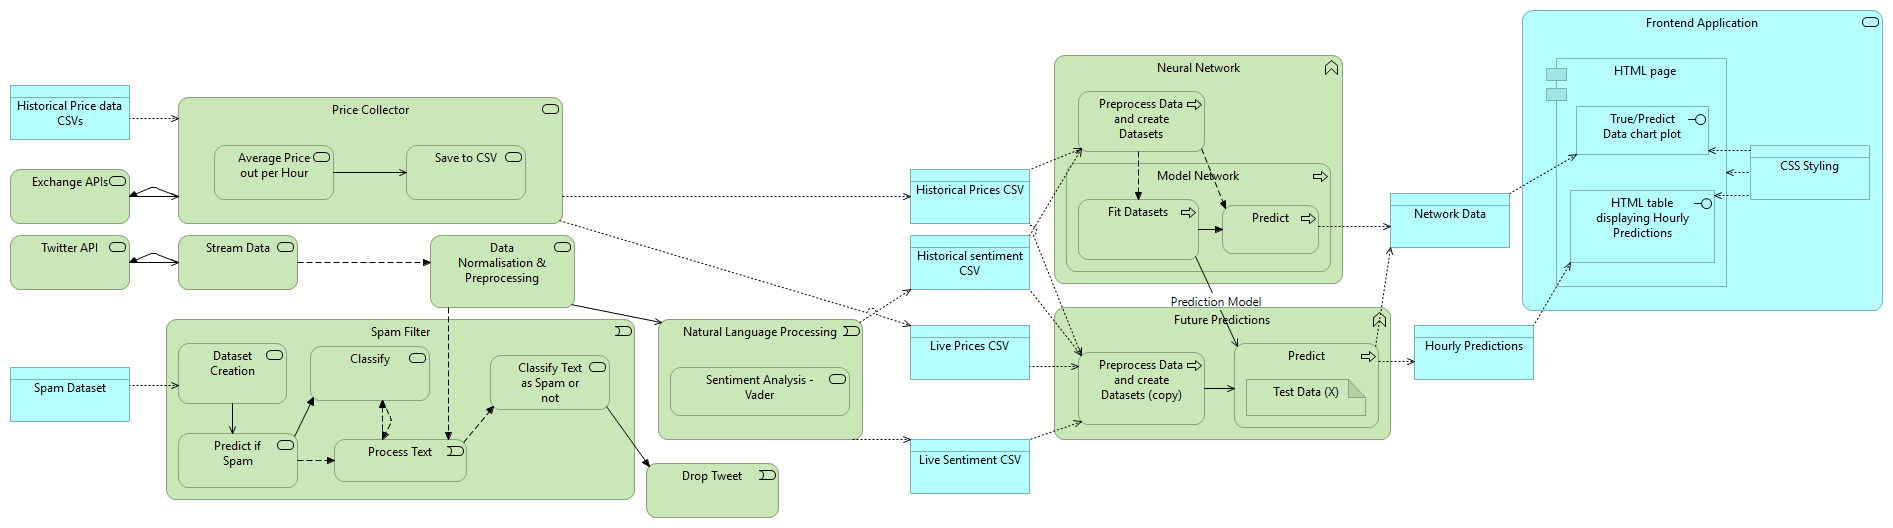
\includegraphics[width=18cm,height=8cm]{images/Generic_Flow.png}
		\begin{center}
			\textit{Figure 4: Basic Dataflow diagram of systems in the project and how data could possibly flow}
		\end{center}
		
	\newpage
	
	\begin{center}	
		\section{System Design}\label{Design}
	\end{center}
		\subsection{Dataflow Designs}
		This section will describe and outline how the system will be formed and will work with each component; a useful way of displaying this is as a dataflow diagram. A dataflow is a way of representing the flow of data through a process or system; as a result, it also provides information about how inputs and outputs of each component work and how they function with other components. It can also give either broad or in-depth overview of the specific workings of each component through how the data is processed and manipulated.
		\newline
		
		\textbf{Dataflow overview of entire system:}
		\begin{center}
			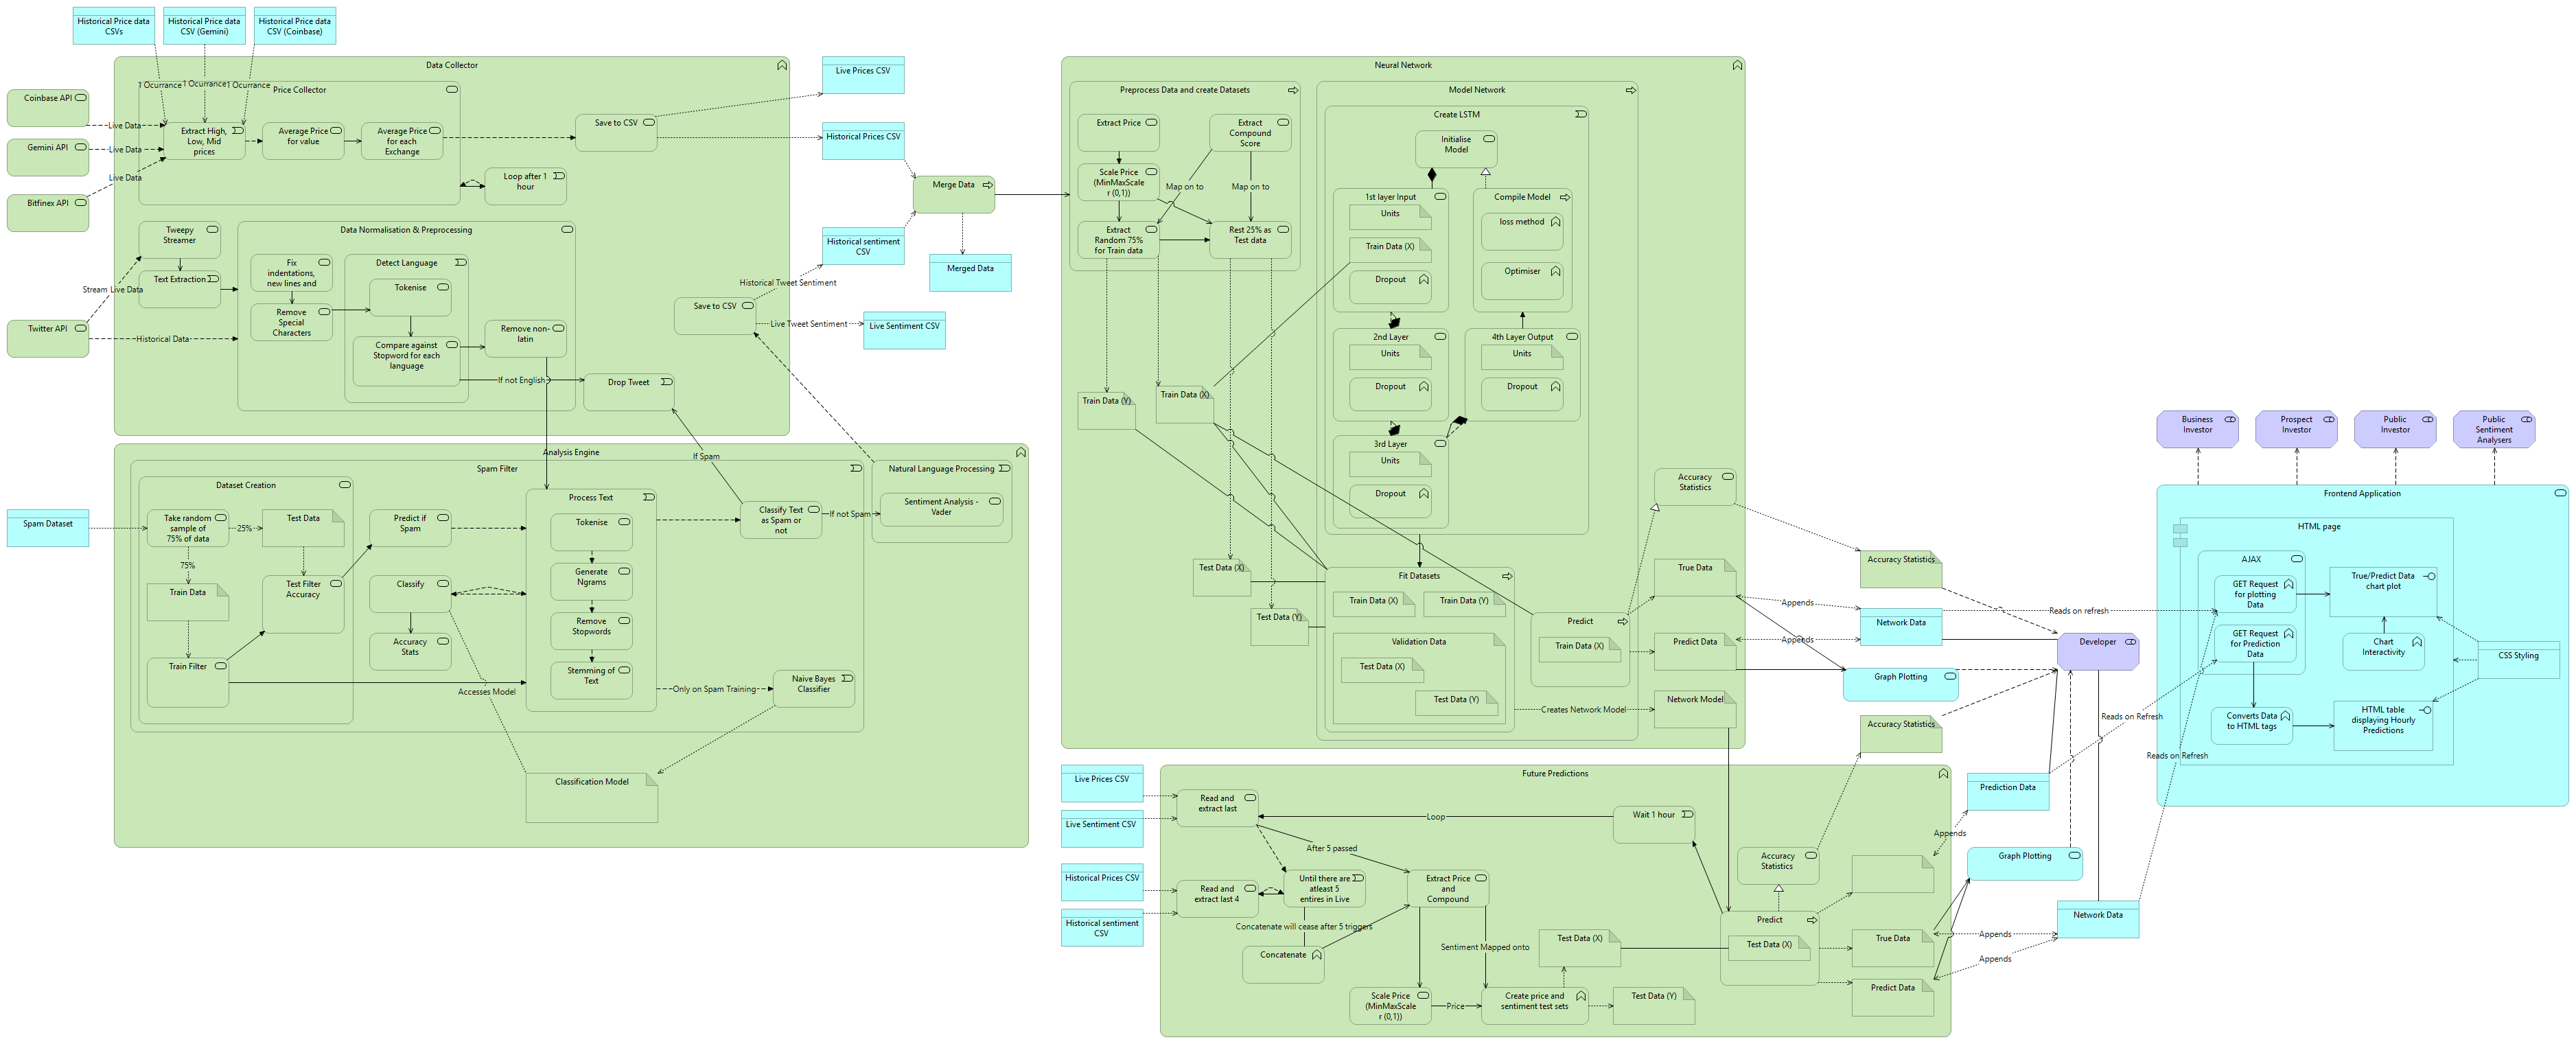
\includegraphics[width=18cm,height=8cm]{images/Dataflow.png}
			\textit{Figure 5: Overall Dataflow diagram of the entire system}
		\end{center}
		This dataflow diagram shows the overall concept of how the data is intended to flow through the system, from being processed and manipulated through each component and what the outputs are of each. Due to the size, this will be broken up and individually explained.
		\newpage
		
		\textbf{Data collector}
		\begin{center}
			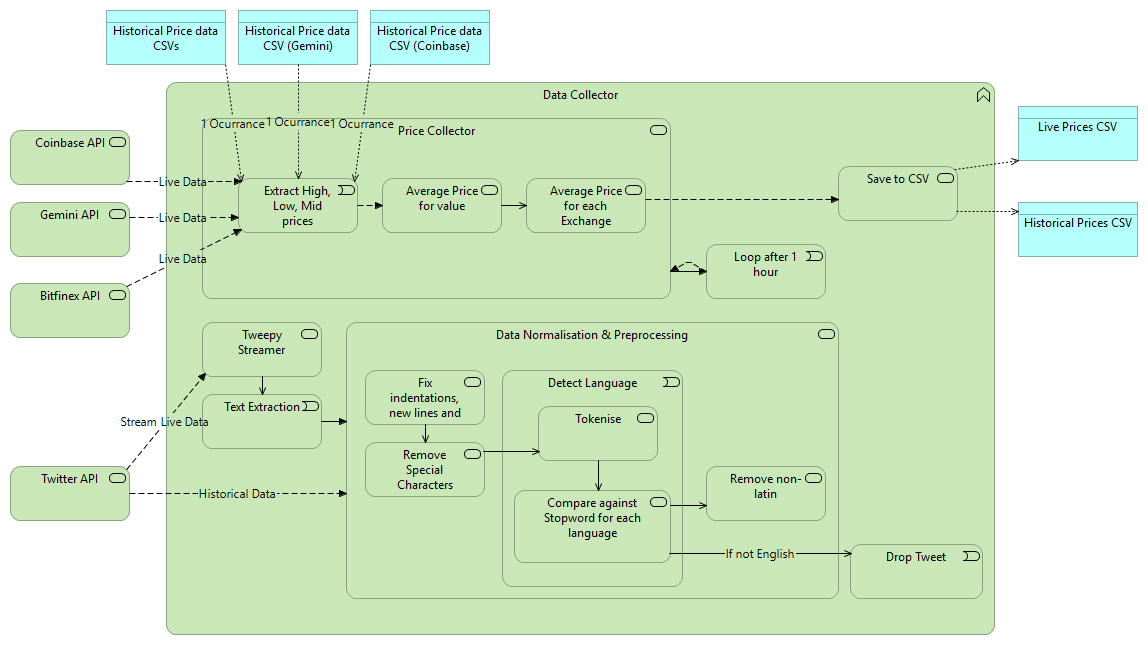
\includegraphics[width=15cm,height=8cm]{images/Data_Collector.png}
			\textit{Figure 6: Data collector Dataflow diagram}
		\end{center}
		This dataflow diagram shows the part of the system responsible for the collection and processing of both historical data. This is split into three parts: Price collector, Tweet collector and tweet normalisation and natural language pre-processing.
		\begin{itemize}
			\item Price Collector - Processes two forms of data, Historical and Live price data. 
			\subitem Historical data is extrapolated from three CSVs that contain the historical price every hour for the past year, from a historical price tracker. At this point in the project, it was identified that historical price trackers do not average the price data from exchanges as previously identified; therefore this data will need to be merged and averaged to create the unbiased hourly price needed. 
			\subitem Live data is extracted directly from the three exchanges APIs shown through REST endpoint requests.
			\subitem Data from both, as separate processes independent from one another, are averaged by extracting the \textit{High}, \textit{Mid} and \textit{Low} hourly prices. This averaged price per hour for each exchange are then averaged together to obtain an unbiased hourly average. The price is then saved to a CSV of historical or live prices respectively. The difference in the flow of data is that of Live prices, in which the process is looped every hour to extract the new hourly prices. 
			\item Tweet Collector - Streams tweets from Twitter using Tweepy, historical tweets are manually collected directly from the Twitter API. Both are fed through the normalisation and data pre-processing stage.
			\item Data pre-processing - This involves cleaning the initial data by removing line breaks and new lines that occur in the data, removal of special characters that are standard in tweets (\textit{'\#','@' and urls}). The data is then fed into a language detection system which tokenises and compares stopwords in the text to NLTK package supported languages. Depending on whether the text is identified as being predominately English or not determines whether or not the tweet is dropped and not used in the network. If the majority is in English, non-English characters are removed as these can still be present in the text.
		\end{itemize}
	
		\textbf{Analysis Engine}
		\begin{center}
			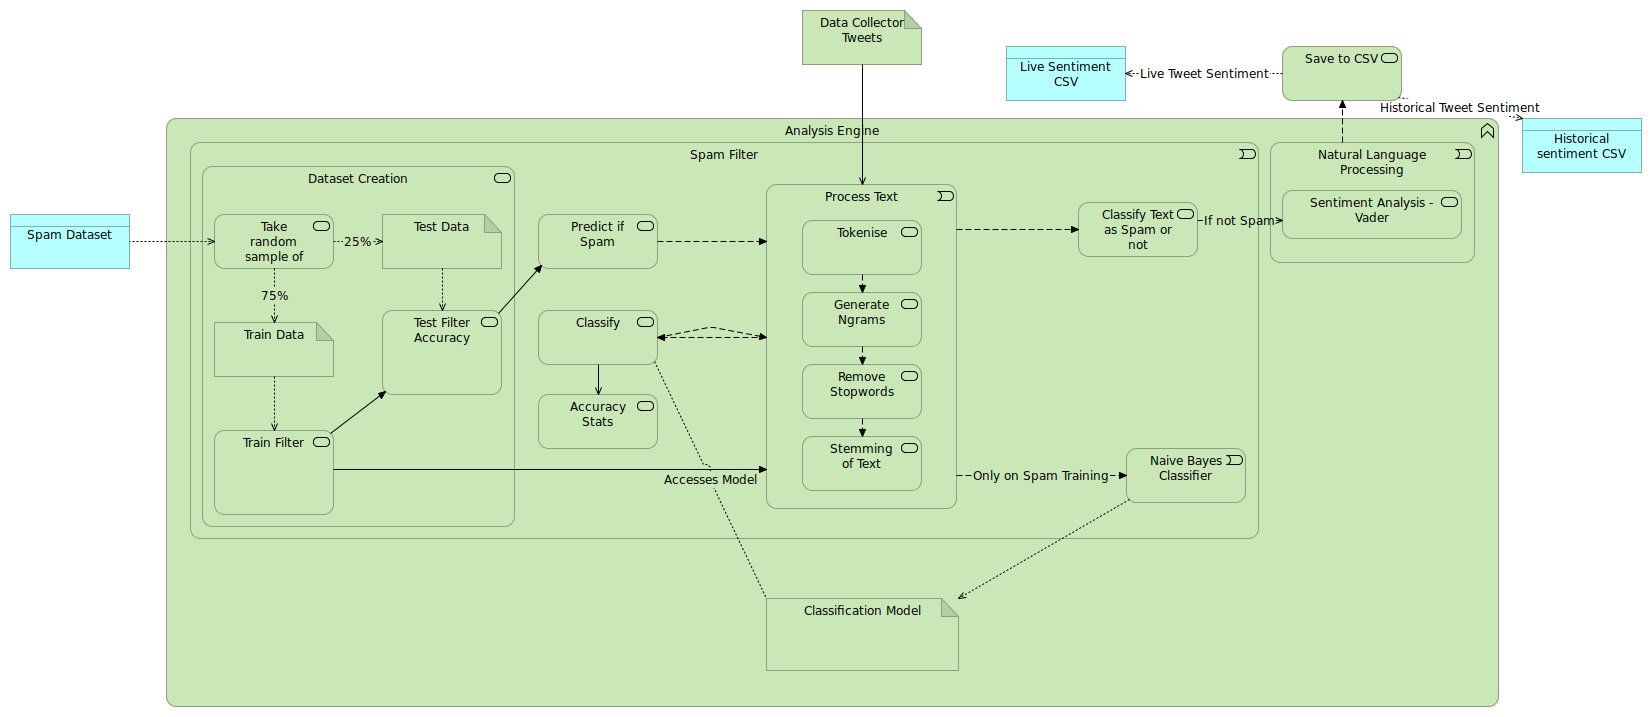
\includegraphics[width=17cm,height=8cm]{images/Analysis_Engine.png}
			\textit{Figure 7: Analysis Engine Dataflow diagram}
		\end{center}
		This dataflow diagram shows the part of the system that is responsible for training a spam filter, creating the model that'll be used to identify if the tweets from the data collector are unwanted - spam. This system is also responsible for assigning the polarity classification to the tweet through sentiment analysis conducted by the VADER package \cite{VADERPaper}.
		\begin{itemize}
			\item Spam filter training - The initial step in this system is to train the Naive Bayes Classifier using the pre-labelled spam dataset which contains an unbiased amount of either spam or ham tweets with their respective labels.
			\subitem This data is split into two samples, training and test sets 75:25 respectively and the Naive Bayes classifier trained and validated against these datasets after pre-processing of the data occurs on the data to prepare it.
			\item Data pre-processing - The tweets from both training and testing the filter and from live and historical tweets are processed through this section. 
			\subitem This section of the system is primarily used to process the tweets for the filter to classify the data and doesn't directly modify the live and historical tweets. The data is processed through various natural language processing techniques such as; Tokenisation, Ngram generation, stopword removal and stemming.
			\item Classifier Modelling and Model creation - Once the data is pre-processed, the data is classified, and the prediction model created, which later used to classify the historical and live tweets.
			\item Sentiment Analysis (VADER) - On a separate route from the spam filter training, using the past and live tweets, the sentiment analyser VADER performs analysis on the tweets and assigns a polarity classification to each text (\textit{Negative, Neutral, Positive} and calculates the compound score which is the difference between the negative and positive ratings \textit{compound}).
			\item Storage - The polarity classification and tweets are then saved to their relevant CSV files for historical and live data.
		\end{itemize}
	
	\newpage
	
		\textbf{Neural Network}
		\begin{center}
			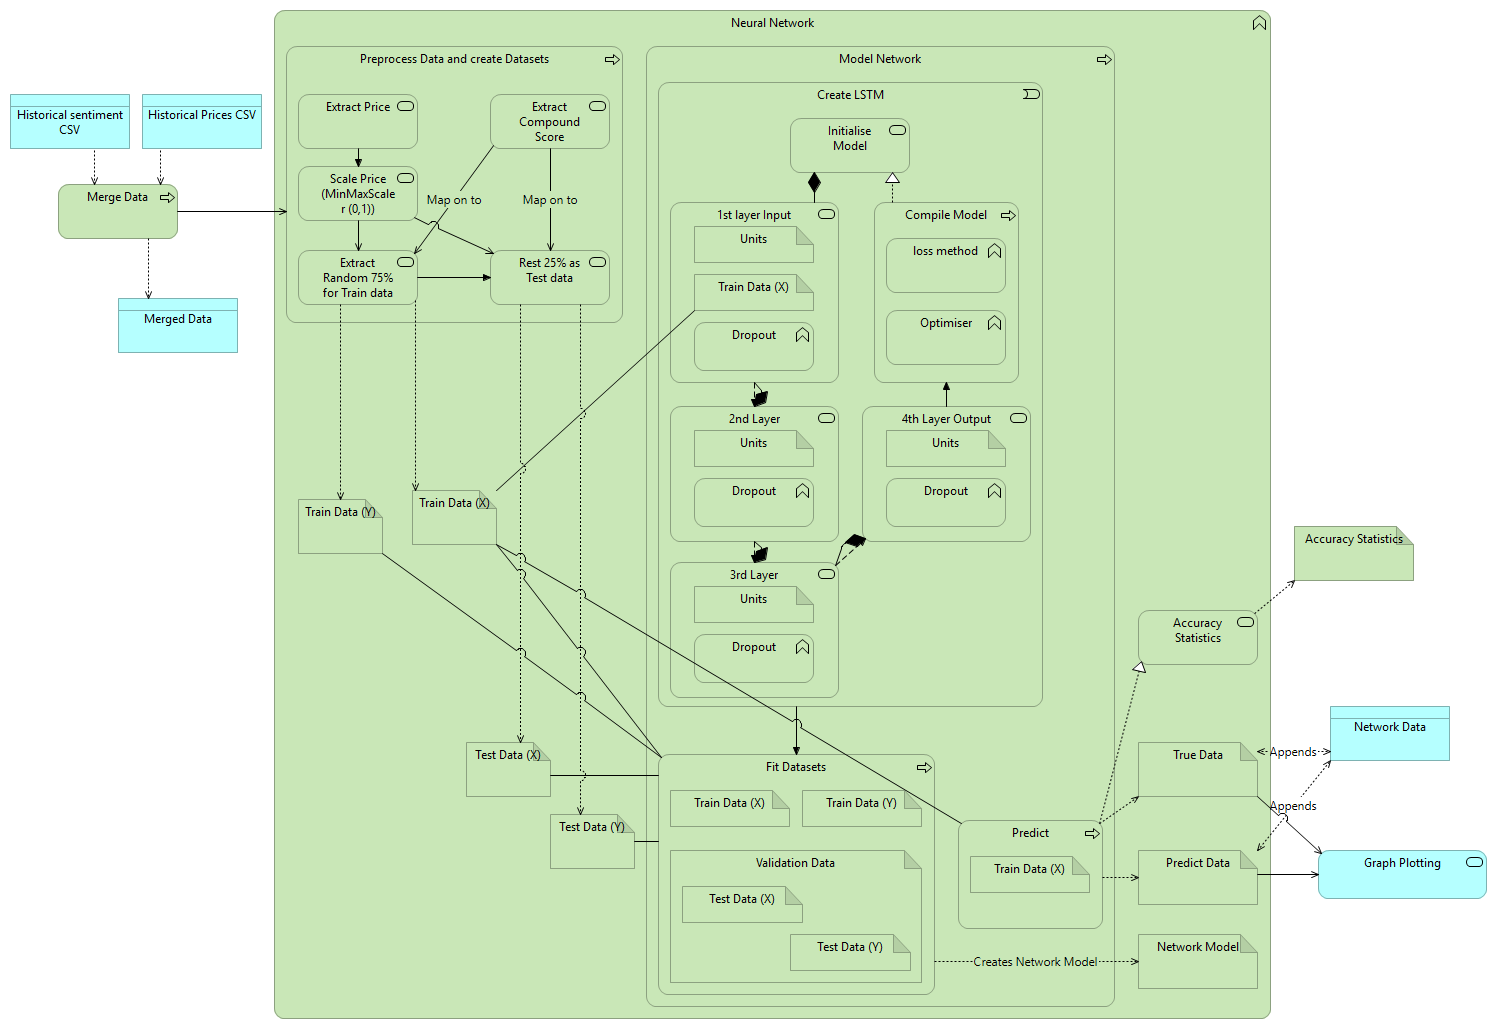
\includegraphics[width=17cm,height=12cm]{images/Neural_Network.png}
			\textit{Figure 8: Neural Network layout Dataflow diagram}
		\end{center}
		The dataflow diagram in \textit{figure 8} shows the part of the system that is responsible for training and creating the neural network model. The dataflow diagram shows how the network will be trained, and the layers of a possible solution to the network. The model shows four layers which may not be the solution that will be implemented but is there to show a representation of a number of layers that could be applied.
		\begin{itemize}
			\item Merging of Datasets - Data from both historical datasets are merged to create one dataset with mapped price and sentiment for each hour. *This is a specific process that is different from the system that does not include sentiment for predictions, the merge process doesn't occur in that system/model.
			\item Training and Testing - Data is split into two samples of training and testing, 75:25 respectively. **This also doesn't occur in the system that doesn't model with the sentiment.
			\item Training network - The training sets, X and Y coordinates are used to train the network.
			\item Testing network - The testing sets, X and Y coordinates of 25\% of the initial data are used to test the validation and accuracy of predictions as these contain the true data of what the predictions should be.
			\item Outputs - Accuracy Statistics, true price data and predicted next hour prices are outputted to respective files for use on the front-end application. The model is then later used for hourly forecasting. 
		\end{itemize}
		
		\textbf{Future Price Forecasting}
		\begin{center}
			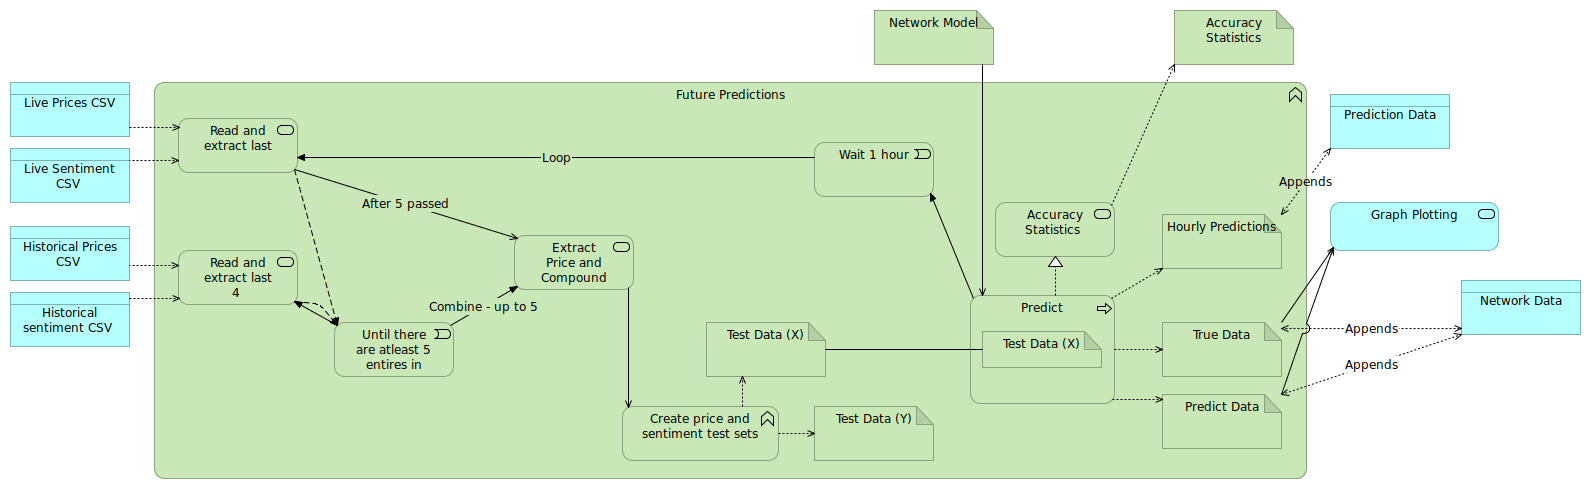
\includegraphics[width=18cm,height=8cm]{images/Future_Predictions.png}
			\textit{Figure 9: Price Forecasting Dataflow diagram}
		\end{center}
		The dataflow diagram in \textit{figure 9} shows how the forecasting system would be implemented. This dataflow shows how it will read live data of both sentiment and price data, merge, split and conduct regression using the trained neural network model to predict the next hour price.
		\begin{itemize}
			 \item Data merging - (Doesn't occur with the system that doesn't include sentiment in price predictions). Data is consolidated from both historical and live data up to 5 iterations. This is due to after the initial hour there will only be a singular record of price and sentiment data, in which no prediction could be made from this as there isn't a sufficient amount of data.
			 \item Prediction - This data is then fitted to the neural network model and predictions for the next time-step hour are made.
			 \item Hour Loop - This will then proceed to loop every hour to make the hourly predictions. Historical price data will cease to be used when there are 5 or more live price records.
			 \item Outputs - Accuracy Statistics, true price data and predicted next hour prices are outputted to respective files for use on the front-end application for charting.
		\end{itemize}
	
		\textbf{Front-end Application}
		\begin{center}
			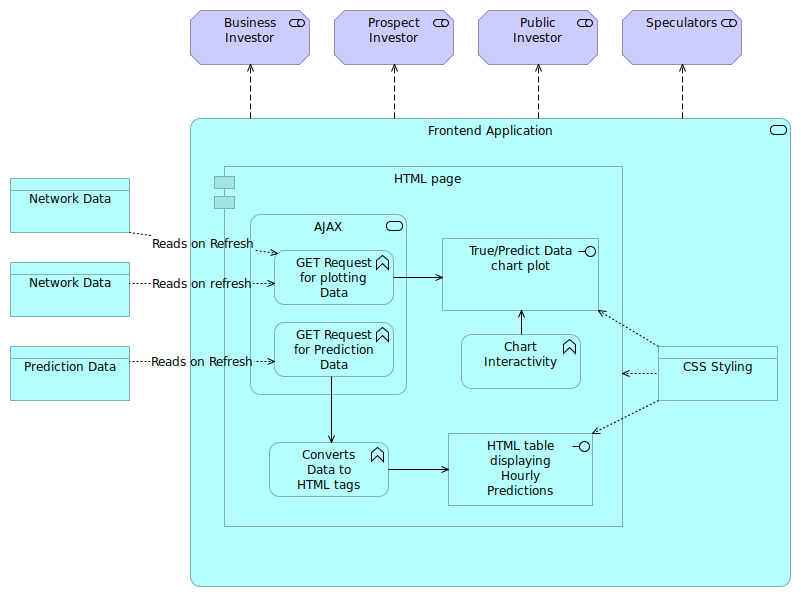
\includegraphics[width=10cm,height=9cm]{images/Frontend_Application.png}
			\newline
			\textit{Figure 10: Front-end Application Dataflow diagram}
		\end{center}
		The above dataflow diagram shows the data flow for the front-end application and how the data is read into the system from the data files generated by the backend application (Neural network).
		\begin{itemize}
			\item AJAX Requests - These are API file requests for files hosted on the server in which the system is running on. This loads the data files into the application for use.
			\item CSS Styling - Contains design styling for page and charts, loaded upon loading of a webpage.
			\item Charting and Tables - Accesses the loaded data from the AJAX requests and plots the data. Prediction data, only with sentiment and prices are plotted into a table. There will be separate charts and tables displaying the data from the backend that hasn't used sentiment in predictions to aid in establishing a correlation between sentiment and price and whether it affects the hourly price (Aiming to solve the problem statement)
			\item Stakeholders - There will be the four stakeholders, outlined in the problem articulation section, that would be the primary users of this application.
		\end{itemize}
		
		\subsection{Interface Design}
	
		\begin{figure}[hbt!]
			\centering
			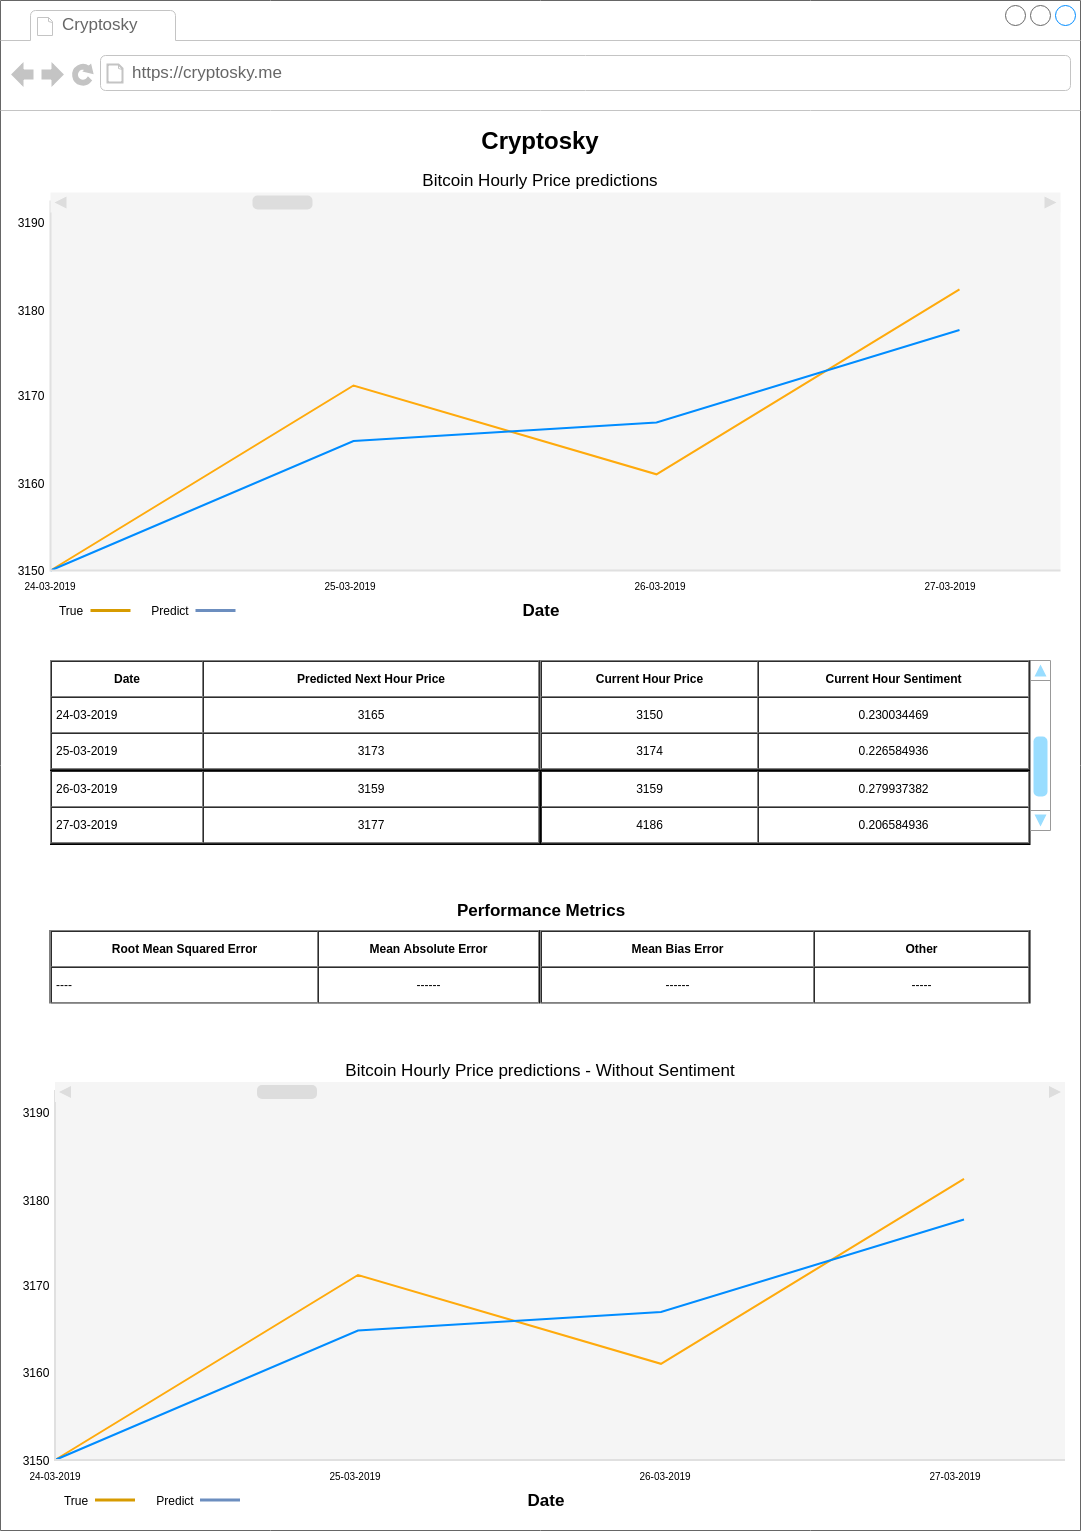
\includegraphics[width=8cm,height=13cm]{images/interface_design.png}
		\end{figure}
		\begin{center}
			\textit{Figure 11: Interface design}
		\end{center}
		\textit{Figure 11} above shows the basic idea of the interface design that will be presented to the stakeholders and aims to be the interface that these stakeholders will use to aid in their market decisions of Bitcoin. The interface, although simplistic, provides all the necessary information that any of these stakeholders would need, it also provides information to allow visual comparison on how sentiment affects the hourly price of Bitcoin, represented as the two charts. The comparison will aid in solving the problem statement later in the conclusion of the project.
		
	\newpage 
	\begin{center}
		\section{Implementation}\label{implementation}
	\end{center}
		This section will outline the method and process of development of the system to satisfy the chosen solution, technical specification and the problem statement. Each section of the system will be outlined and discussed with relevant codes snippets of essential methods from the system to highlight the processing of data throughout. Additionally, the order in which the following sections are show was not the order in which they were developed, the order in which they are shown is to represent the order of how the data flows through the system, see \textit{section 9 - System Design} for an understanding of the flow of data through the system.
		\newline
		
		\subsection{Data collection}\label{collection}
			\subsubsection{Price Time-Series Historical Data}
			Historical price data was extracted from a CSV historical price tracker, \textit{Bitcoin Charts} \cite{btcCharts}. This tracker provided the historical data from the three exchanges used for Live price collection - Coinbase, Bitfinex and Gemini, since the exchanges supported the cryptocurrency. The data used spans from \textit{2018-01-06} to \textit{2019-01-06}.
			
			\begin{lstlisting}[language=Python, caption=Historical price collection and averaging per exchange]
...
coinbase = pd.read_csv('coinbase_btcusd.csv')
bitfinex = pd.read_csv('bitfinex_btcusd.csv')
gemini = pd.read_csv('gemini_btcusd.csv')
			
coinbase.drop(columns=["Currency", "24h Open (USD)", "24h High (USD)", "24h Low (USD)"], axis=1, inplace=True)
			
coinbase.columns = ["timestamp", "price"]
			
coinbase['timestamp'] = pd.to_datetime(coinbase['timestamp'])
			
coinbase = coinbase.set_index('timestamp').resample('1D').mean().resample('1H').mean()
... # similar code for the other 2 exchanges
			
data.set_index(coinbase['timestamp'])
for i in data:
	data['price'] = (coinbase['price'][i] + gemini['price'][i] + bitfinex['price'][i])/3
			
data = data.fillna(method='backfill')
data = data.round(3)
			\end{lstlisting}
			
			Due to each of the hourly prices in each CSV for each exchange were averaged from the \textit{'high'}, \textit{'mid'} and \textit{low} prices, the data from each exchange only needed to be averaged together. This data is averaged and then saved to a CSV containing historical prices of Bitcoin for the past year.
			
			\subsubsection{Price Time-Series Live Data}
			Live price data, as described in the solution approach, were extracted every hour from three exchanges - Coinbase, Bitfinex and Gemini were chosen for providing this data due to being the most popular exchange platforms that provide an API for retrieving live price data.
								
			The \textit{'high'}, \textit{'mid'} and \textit{low} prices were extracted from the endpoint response and averaged to provide an overall hourly price per exchange.
			
			\begin{lstlisting}[language=Python, caption=Extraction of Price from exchanges]				
def coinbase():
	...				
	try:
		client = Client(api_key, api_secret)
		repsonse = client.get_spot_price(currency_pair = 'BTC-USD')
		price = (float(repsonse['amount']))
		price = round(price, 3)
		return price
	except KeyError as e:
		print("Error: %s" % str(e))
		sys.stdout.flush()
		price = 0
		return price
				
def bitfinex():
				
	try:
		response = requests.request("GET", "https://api.bitfinex.com/v1/pubticker/btcusd")
		response = json.loads(response.text)
				
		price = (float(response['low'])+ float(response['mid']) + float(response['high']))/3
		price = round(price, 3)
		return price
	except KeyError as e:
		print("Error: %s" % str(e))
		sys.stdout.flush()
		price = 0
		return price
				
def gemini():
	... # Exact code to bitfinex()
			\end{lstlisting}
			
			The above code shows how this was implemented as a system for the price extraction from the APIs.
			
			These functions are called every hour by a master function which uses the averaged price from each exchange to average and creates a fair, unbiased hourly price, which is the saved to a CSV containing the live unbiased price for the hour along with the time of creation. The function also checks if an error state is returned from any of the exchange functions and sets the default price to zero, instead of averaging the three exchanges only the responses that successfully returned a price are averaged.
					
			
			\subsubsection{Historical Tweet Collection}
			Historical tweets were obtained directly from the Twitter API through a simple Curl command for the given date range of the past year. Multiple accounts were created to obtain the amount of data needed, as detailed in the data gathering section under the solution approach. Due to the vast amount need, 5 tweets averaged per hour for the past year would require 1.2 requests per day (40320 total to get a whole year's worth), totalling 9,050,000 tweets. As this was highly unfeasible with the API access available for this project, 1 tweet per hour (25 per day, 1 request per 4 days) was obtained rather than the average, which resulted in only ~92 requests needed to get the required data. 
			
			\begin{lstlisting}[language=, caption=Sample Curl request - data saved to json and python scripted called to process data]
curl --request POST \
	--url https://api.twitter.com/1.1/tweets/search/fullarchive/boop.json \
	--header 'authorization: Bearer TOKEN' --header 'content-type: application/json' \
	--data '{"query": "bitcoin", "maxResults":100, "fromDate":"201904050000", "toDate":"201904050200"}' -o data_collector/twitter/temp_hist_tweets.json \
	&& python3 data_collector/twitter/sift_text.py
			\end{lstlisting}
			
			These tweets are processed through the spam filter to detect if they were included unwanted text, cleaned and a polarity classification assigned to each for each hour. The process of how both the spam classification, pre-processing of the data and polarity classifications work will be detailed in their relevant sections of the system below.
			
			\begin{lstlisting}[language=Python, caption=Sift-text python script - used alongside Curl command in Listing 4]
import tweet_collector	## pre-processing functions
import spam_filter			## spam filter classification
import analysis_engine.sentiment_analysis as sentiment_analysis	
## Sentiment analysis and polarity classification (symbolic link to file)
			
def processTweet(tweet, tweetFilter):
			
	now = datetime.datetime.now()
				
	#Data preprocessing
	removedLines = tweet_collector.utilityFuncs().fixLines(tweet)
	removedSpecialChars = tweet_collector.utilityFuncs().cleanTweet(removedLines)
	removedSpacing = tweet_collector.utilityFuncs().removeSpacing(removedSpecialChars[0])
	tweetLength = tweet_collector.utilityFuncs().checkLength(removedSpacing)
			
	if tweetLength == True:
	## Drop tweet if too short
				
		##Check if the tweet is predominantly English				
		checkIfEnglish = tweet_collector.utilityFuncs().detectLaguage(removedSpecialChars[0])
			
			
		if checkIfEnglish == True:
			## Remove non-English Characters
			tweetText = tweet_collector.utilityFuncs().remove_non_ascii(removedSpacing)
			print("Cleaned Tweet: ", tweetText)
			sys.stdout.flush()
			
			cleanedTweet = tweetText+' '+removedSpecialChars[1]
			
			## Check with spam filter - drop if classified as spam
			classification = tweetFilter.testTweet(cleanedTweet)
			
			if classification == False:
				## Perform Sentiment Analysis
				ovSentiment, compound = analyser.get_vader_sentiment(cleanedTweet)
							
				try:
					## Save to historical tweets file
					with open('data_collector/historical_tweets.csv', mode='a') as csv_file:
						writer = csv.DictWriter(csv_file, fieldnames=['created_at', 'tweet', 'sentiment', 'compound'])
						writer.writerow({'created_at': now.strftime("%Y-%m-%d %H:%M"), 'tweet': cleanedTweet, 'sentiment': ovSentiment, 'compound': compound})
						return True
				except BaseException as exception:
					print("Error: %s" % str(exception))
					sys.stdout.flush()
					return False
			else:
	.... # other finished else statements with print statements
			\end{lstlisting}
			
			As detailed in the comments for the code, this function conducts external functions and data manipulation on the data, most of which are predefined in the \textit{tweet\_collector.py} script. These are not redefined in this function to reduce code duplication throughout the system and hence are imported at the beginning of the file. Due to the nature of spam filtering tweets were inevitably removed; therefore a few hours of data were missing. This was resolved by making another request for that specific hour and averaging the sentiment for the given hour to fill missing data.
			
			\subsubsection{Live Tweet Collection}
			Live tweets were obtained through the use of the Tweepy package to stream current tweets per hour from the Twitter API. Spam filter detection, data pre-processing and language detection are also conducted on this data and are defined within this python script \textit{'tweet\_collector.py'}, these functions are described in the relevant sections in the Data processing section.
			
			On the initial running of the \textit{'tweet\_collector.py'} script the CSV files for storing tweets and tweets are initialised, which will contain the polarities assigned by the VADER analyser. More importantly, it initialises the spam filter and trains it based on the pre-labelled spam dataset.
			
			Functions used for training relate to relevant functions defined under the \textit{filterSpam} class which are used to create the training and test datasets. This function is described in the Spam Filtering section below.
			
			The streaming of tweets are handled by the Tweepy package and is first initialised upon starting of the python script. The streaming method works by establishing a listener and authenticated with the Twitter API; it then listens on that connection for data. This streamer can also filter on language and a specified hashtag which is loaded from a \textit{'.env'} file also containing the API keys for authentication.
			\newline
			
			
			\begin{lstlisting}[language=python, caption=Tweepy Streamer setup]
	class Streamer():				
		def stream_tweets(self, tweets_file, temp_tweets, hashtag, tweetFilter, analyser):
			listener = Listener(tweets_file, temp_tweets, tweetFilter, analyser)
			auth = OAuthHandler(keys().api_key, keys().api_secret)
			# Load API keys from env file and set auth
				
			print("Console: ", "Authorising with twitter API")
			sys.stdout.flush()
				
			auth.set_access_token(keys().access_token, keys().access_secret)
			# Set access keys
						
			print("Console: ", "Streaming Tweets")
			sys.stdout.flush()
				
			stream = Stream(auth, listener, tweet_mode='extended')
			stream.filter(languages=["en"], track=hashtag)
			## Execute streamer and filter for only English region tweets and by specified hashtag ('Bitcoin')
			\end{lstlisting}
			
			Once the listener and streamer are declared, and Tweepy begins listening all data is processed through the \textit{on\_data} method. In this function, the tweet is extracted from the response and performs data pre-processing, language detection, spam classification and sentiment analysis on the data. Additionally, there is an initial time interval that checks for a time limit - this is used to ensure that the script runs for just under an hour and restarts every hour. This allows the average of the gathered tweets' sentiment to be summed for that hour and then used for the network price predictions. 
			
			The tweet text can be nested in multiple attributes in the response; this depends on a few factors of what the tweet is and how it was posted on Twitter. If a user retweeted the tweet, the text of the tweet would be nested under \textit{'retweeted\_status'} in the JSON response, also there is a check to see if the tweets are above the original twitter tweet character limit (140 characters). This is a possible legacy parameter in the Twitter API but is checked upon data response. If an attribute \textit{'extended\_tweet'} exists the character limit for the tweet exceeds 140 but is under the 280 characters hard limit of Twitter, this exact filtering is the same if it in a non-retweeted tweet.
			
			As for the key facts about this function; the length of the tweet is checked to be above 5 (tokenised) due to any tweets with fewer words will not contain enough information to be given a proper polarity classification and almost always returns as 100\% neutral, which is of no use and will have no effect on the hours average sentiment. The entire code in the function is encapsulated in a try-catch to check if data was received and handles non-responses and missing data. If there was no data the issue is ignored unless a connection between the streamer and API is broken it otherwise exits the script. As for the processing of the tweet the code in \textit{Listing 4} is used.	
			
			\newpage
		\subsection{Data pre-processing}\label{processing}
			
			Various techniques and tools have been utilised throughout the development of the system to process the data appropriately so it can be parsed by VADER, spam filter and neural network. This section will cover the crucial functions that provide such functionalities and that are called throughout the system, as seen in some of the above code snippets.
			
			\subsubsection{Tweet Filtering}
			
			Various 'Utility Functions' have been used to initially filter out unwanted data from tweet text. These functions called by, both live tweet (\textit{tweet\_collector.py}) and historical tweet (\textit{sift\_text.py}) processing, prior any polarity classification or storing of tweet data to CSV files.
				
				\begin{lstlisting}[language=python, caption=Basic data filtering and processing function - defined in 'tweet\_collector.py']
	def cleanTweet(self, text):
		# Function to clean tweets, removes links and special characters
		return re.sub(r'([^0-9A-Za-z \-\%\£\$ \t])|(@[A-Za-z0-9]+)|(http\S+)', '', text), ' '.join(c for c in text if c in ji.UNICODE_EMOJI)
		# Also removes emojis from text - later re-added due to VADER supporting emoticons
				
	def removeSpacing(self, text):
		return re.sub(r'( +)', ' ', text)
		# Removes extra spacing that may be left between words
				
	def fixLines(self, text):
		return re.sub(r"([\r\n])", " ", text)
		# Removes line breaks and new lines from text
								
	def remove_non_ascii(self, text):
		return ''.join(i for i in text if ord(i)<128)
		# User after language detections and removes non-English characters from text
		
	def checkLength(self, text):
		tokens = text.split()
		if len(tokens) <= 5:	# Tokenisation
			return False
		else:
			return True
				\end{lstlisting}
				
		    Due to VADER being a lexicon-based sentiment analyser little data pre-processing needs conducting on the tweet text. The functions above primarily remove unnecessary text from the tweet that will either provide no insight into public opinion or can obstruct a proper classification of the sentiment - such as the existence of URLs in the given text. Additionally, the 'clean\_tweet' function removes the emojis in the given text if any are presently using the emoji package - which in turn is another lexicon that compares the given text to any emoticon contained within the lexicon. These are removed at this stage but are later re-added back to the text as VADER support emoticon classification. 
		    The last function in 'utility functions', 'checkLength' splits the text up into individual words (tokens - a process of tokenisation), this is used to check the total length of a tweet. If the tweet is less than five words, it is dropped from classification. This is due to text containing less than five words are less likely to produce a meaningful polarity classification than texts above that word limit. Additionally, any meaningful information is unlikely to be forced into five words.
			
			\subsubsection{Language detection filtering}
			
			The language detection feature of the system is used as an additional filter for filtering out non-English tweets. As discussed in the solution approach, Tweepy/Twitter API provides a means to filter out non-English based tweets. This, however, will not work if the user has settings on Twitter such as the prefered language and the region set to be English. Due to this, non-English characters can still be contained within the collected tweets; thus these are detected and filtered with the language detection function.
			
			\begin{lstlisting}[language=python, caption=Language detection and filter function \cite{langdectNLTK}]
def detectLaguage(self, text):
	...
	
	# Split words up into tokens - tokenisation
	tokens = wordpunct_tokenize(text)
	
	# Shift to lower case
	words = [word.lower() for word in tokens]

	# Compute per language in nltk number of stopwords in text
	for language in stopwords.fileids():
		stopwords_set = set(stopwords.words(language))
		words_set = set(words)
		common_elements = words_set.intersection(stopwords_set)

		language_ratios[language] = len(common_elements) 
		# Form ratio scores for each language detected from stopword comparison

	ratios = language_ratios
	highest_ratio = max(ratios, key=ratios.get)
	# Extract highest ratio language used in given text

	print("Console: Text is - ", highest_ratio)
	sys.stdout.flush()

	if highest_ratio == 'english':
		return True
	else:
		return False
	# If text is not predominately English drop tweet
			\end{lstlisting}
			
			The language detection function uses several natural language pre-processing techniques to identify the most predominant language for the given text. This is accomplished by first tokenising the text into tokens and converting them to lower case - this is so that the stopwords can be identified. For each of the languages supported by the Natural Language Toolkit Python package, the stopwords are identified in the text and compared to the stopwords in the language corpus' in NLTK. The ratios for the individual languages are formed, and then the predominant language identified. If the language is not predominantly English, the tweet is dropped. 
			
			There is however an issue with this approach, if a tweet contains too many special characters - characters that are allowed, the tweet occasionally is not classified as English even when it predominantly is upon visual inspection; therefore the tweet is dropped and not processed. This isn't a significant issue as about 3000 tweets can be collected in an hour, and some of these would be filtered out by the spam filter regardless.
			
			Additionally, an n-gram method could be used to distinguish the language of the given text and may perform more accurately than the word-based approach that was implemented \cite{LanNgram}. This could be a later improvement, as the n-gram approach requires a corpus for each language to compare against to be presented, the word-based approach is sufficient for its use case. Therefore it could be used as a comparison between approaches and seen as a possible improvement at a later date.
			
			\newpage
			
			\subsubsection{Spam filter - Tokenisation, Ngrams, Stopword removal and Stemming}
			
			Prior to any text being processed to both train the Naive Bayes classifier of the spam filter or to classify live tweets, the data needs to be pre-processed to extract the feature vetors from the text, so that the classifier can identify the probability of each word in the given text. The explanation of how this classifier functions will be detailed in the 'Spam Filtering' Section.
			
			\begin{lstlisting}[language=python, caption=pre-processing of data prior to being used by the spam filter]
def processTweet(tweet, gram = 2):
	tweet = tweet.lower() # convert to lower case
				
	words = word_tokenize(tweet)    # Tokenise words in text
	words = [w for w in words if len(w) > 2]  
	# remove words that are not greater than 2 characters
				
	if gram > 2:    ## Increasing grams can increase accuracy
		w = []
		for i in range(len(words) - gram + 1):
			w += [' '.join(words[i:i + gram])]
		return w
				
	# Remove stopwords
	sw = stopwords.words('english')
	words = [word for word in words if word not in sw]
	# Create new dict without stopwords
				
	stemmer = PorterStemmer()           # Stem words
	words = [stemmer.stem(word) for word in words]
	# Create new dict of stemmed words
				
	return words
			\end{lstlisting}
			
			The actions performed on the text consist of:
			\begin{itemize}
				\item Convert to lower case: This is due to that 'DROP' and 'drop', and likewise words convay the same meaning thus these are simply converted to all lower case.
				\item Tokenise words: This splits the text into individual words. A dictionary is then created from the tokens that are above the length of 2 - due to words that are of less 'is', 'he' and 'if' will not contribute to spam detection and are seen as generic words in the English language
				\item Ngrams: This is implemented to provide richer word sequences for the spam filter classification, as explained in the litrature review use of ngrams can increase accuracy.
				\item Stop words Removal: This removes stopwords such as 'this', 'we' and 'now' from the text. Due to these common words carrying less importance for sentiment analysis.
				\item Stemming: Reduces words down to their smaller form, as in it remove suffixes from inflected words - 'studying' become 'study' \cite{StemvsLem}. The Porter Stemmer works by removing the suffixes from the text - 'going' becomes 'go', however, this applies to other words such as 'leaves' becomes 'leav' which is not a word. However, this method will be applied equally to all words containing such suffixes so all variations will become so, thus still allowing the probability classifications to occur on the word as all variations will be the same. 
			\end{itemize}
			
			As discovered from \cite{StemvsLem}, lemmatisation could be an alternative and arguably a better solution to stemming. Lemmatization works fundamentally the same as stemming but reduces the inflected words properly ensuring that a root word belongs to a language. Using the same words that are used to describe stemming, lemmatisation reduces 'goes' to 'go' and 'leaves' to 'leaf' as an example - by removing the suffixes down to create the actual root word.
			Although lemmatisation will provide the classifier with an actual English word, stemming regardless still reduces the words down to a similar form, this added with a lemmatiser needing a corpus for classifying the words to their root words and additional computational time to do so, the former of using a stemmer is sufficient for the use case.
			
		\subsection{Spam Filtering}
			This section of the implementation will describe how the spam filter is initialised in the \textit{tweet\_collector}, how it is trained and how it classifies tweets as being either spam or ham (wanted data).
			
			The function is initialised within the \textit{tweet\_collector}, that creates the training and testing datasets, and tests classifier on hard specified tweets and checks their classification.
			
			\begin{lstlisting}[language=python, caption=Spam filter training Class - \textit{tweet\_collector.py}]			
class filterSpam(object):		
...		
def trainFilter(self):
	self.dataset()		## Split dataset 75:25
	self.train()		## Train based on training dataset
			
def dataset(self):
	self.data = pd.read_csv(self.training_set)
			
	self.data['class'] = self.data['classes'].map({'ham': 0, 'spam': 1})
	# Remap labels of 'Spam' and 'Ham' to 1:0 respectively
			
	self.data.drop(['classes'], axis=1, inplace=True)
	# Drop old labels
			
	self.trainIndex, self.testIndex = list(), list()
	for i in range(self.data.shape[0]):
		if np.random.uniform(0, 1) < 0.75:	# Random shuffle data of 75%
			self.trainIndex += [i]	# Create training index
		else:
			self.testIndex += [i]	# Create testing index
	self.trainData = self.data.loc[self.trainIndex]
	self.testData  = self.data.loc[self.testIndex]
	# Define datasets by getting values from first 75% and then 25%
			
	self.trainData.reset_index(inplace=True)
	self.testData.reset_index(inplace=True)		
	# Reset indexes
			
	self.trainData.drop(['index'], axis=1, inplace=True)
	self.testData.drop(['index'], axis=1, inplace=True)
	# Drop old index
			
def train(self):
	self.spamFilter = spam_filter.classifier(self.trainData)
	# Initialise the spam filter with the 75% dataset
			
	self.spamFilter.train()
	# Train
			
def testData_Prediction(self):
	# Classify data from test dataset
	prediction = self.spamFilter.predict(self.testData['tweet'])	
	return prediction
			
def testPrediction(self):
	# Test Spam/Ham tweets - should return True and False respectivly
	spam = spam_filter.processTweet("Earn more than 0015 btc free No deposit No investment Free Bitcoins - Earn $65 free btc in 5 minutes bitcoin freebtc getbtc")
			
	ham = spam_filter.processTweet("Bitcoin closed with some gains in month of February")
	# Process Tweets - Tokenise and Stem
					
	hamTweet = self.spamFilter.classify(ham)
	spamTweet = self.spamFilter.classify(spam)
	# Classify both tweets

def filterStatistics(self, prediction):
	# Get performance metrics for prediction data compared to actual test data
	spam_filter.metrics(self.testData['class'], prediction)
			
def testTweet(self, tweet):
	# Used for live tweets classification
	processed = spam_filter.processTweet(tweet)
	classified = self.spamFilter.classify(processed)
	
	return classified
			\end{lstlisting}
		
		\begin{itemize}
			\item trainFilter: is a function that calls the dataset function which created the training and testing dataset, followed by the train function which trains the initialised classifier. This function's sole purpose is to serve as a parent function that only needs to be called to perform the child functions once.
			\item dataset: This function loads the pre-labelled spam dataset, remaps the labels to integers 0:1 to ham:spam respectively, creates a dictionary with an index of 75\% of the original data for the training dataset and 25\% for the testing dataset. This function does this by extracting the data at the set point from the spam dataset into the relevant new datasets which resetting indexes and dropping old columns to form appropriate data.
			\item train: Is used to call the classifier function defined in the \textit{spam\_filter} script and passes the training data for it to initialise then train on.
			\item testData\_Prediction: Is a function similar to the 'train' function, but calls the 'predict' function defined in \textit{spam\_filter} to test the classifier on the test data and returns the predictions made, which is used later on in the 'filterStatistics' function to calculate the accuracy of the classifier.
			\item testPredictions: This function is used to test the accuracy of the trained classifier with pre-defined tweets that are assumed to be either spam or ham. The primary goal of this function is to ensure that the classifier correctly classifies the two tweets as either spam or ham appropriately. The text is processed through the 'processTweet' function previously described to transform the tweets into tokens ready for classification.
			\item filterStatistics: Is used by the 'testData\_Predictions' function to calculate the accuracy of the classification model using the test data and prediction data. The 'metrics' function is defined in the \textit{spam\_filter} script.
			\item testTweet: Is a function used on the live tweets by the 'on\_data' function also outlined previously to process the tweets data and classify it as either being spam or not, the 'on\_data' function then handles the result accordingly.
		\end{itemize}		
		
		\subsubsection{Naive Bayes model}
		
		The spam filter classifier, using a Naive Bayes model, was coded from scratch. This was ultimately unneeded as the Scikit-learn python package comes with four inbuilt Naive Bayes classification models (Bernoulli, Complement, Multinomial, Gaussian)\cite{NValgor}. The model was coded from scratch due to finding information on how this would be done with techniques such as TFIDF and Additive Smoothing as detailed in the literature review, the tutorial that helped the greatest \textit{Spam Classifier in Python from scratch} \cite{SpamCScratch} \cite{SpamOrHamGit}. For an explanation of how the maths work behind this classifier see Literature review sections 'Bag Of Words', 'TF-IDF' and 'Addictive Smoothing'. 
		
		The Naive Bayes model implemented was a multinomial Bayes model as the data used for classification was of multinomial distribution and categorical. This algorithm was not compared to the Scikit-learn's inbuilt model for accuracy as this was not the focus of this project. 
		
		\begin{lstlisting}[language=python, caption=classifer class of spam\_filter.py]
def TF_and_IDF(self):
...
	# Bag Of Words implementation 
	
	for entry in range(noTweets):
		processed = processTweet(self.tweet[entry])
		count = list() 
	#To keep track of whether the word has ocured in the message or not. TF count
		for word in processed:
			if self.labels[entry]:
				self.tfSpam[word] = self.tfSpam.get(word, 0) + 1
				self.spamCount += 1	
				## If label for data is spam then add words to spam list
			else:
				self.tfHam[word] = self.tfHam.get(word, 0) + 1
				self.hamCount += 1
				# If label for data is ham then add words to ham list
			# Addictive Smoothing - if current word is not seen add count list
			if word not in count:
				count += [word]
		for word in count:
		# Loop unseen word list
			if self.labels[entry]:
				self.idfSpam[word] = self.idfSpam.get(word, 0) + 1
			else:
				self.idfHam[word] = self.idfHam.get(word, 0) + 1

def TF_IDF(self):
...
	# Calculate probability of word being spam or ham based on occurance in text compared to counted sets along with relevant keys
	for word in self.tfSpam:
		self.probSpam[word] = (self.tfSpam[word]) * log((self.spam + self.ham) / (self.idfSpam[word] + self.idfHam.get(word, 0)))
		self.sumSpam += self.probSpam[word]
	
	for word in self.tfSpam:
		self.probSpam[word] = (self.probSpam[word] + 1) / (self.sumSpam + len(list(self.probSpam.keys())))
	
	for word in self.tfHam:
		self.probHam[word] = (self.tfHam[word]) * log((self.spam + self.ham) / (self.idfSpam.get(word, 0) + self.idfHam[word]))
		self.sumHam += self.probHam[word]
	for word in self.tfHam:
		self.probHam[word] = (self.probHam[word] + 1) / (self.sumHam + len(list(self.probHam.keys())))
		
		# Calculate total amount of spam words identified
		self.probSpamTotal, self.probHamTotal = self.spam / self.total, self.ham / self.total
		\end{lstlisting}
		
		\subsubsection{Classification}
		
		The classification function aims to classify the pre-processed tweet data as either spam or ham based on the term-frequency and probabilities calculated in the 'TF\_IDF' function. This conducted for each word in the processed tweet is identified if the word is contained in the spam set, based on the level of occurrence the probability is assigned a weight (The more it occurs, the more likely it is a generic word), this is also identified for the level of occurrence in the ham set. Totals for the probability are formed, and the total count for both spam and ham are added to the spam and ham probabilities for the processed tweet. If the spam probability \textit{pSpam} is higher than the ham probability \textit{pHam} based on the level of occurrence of each word in the modelled respective sets, a boolean is returned based on which probability is higher - which identifies if the tweet is predominantly spam or ham (\textit{True} or \textit{False}).
		
		\begin{lstlisting}[language=python, caption=Classify Function of Parent classifier class of spam\_filter.py]
def classify(self, processed):
	pSpam, pHam = 0, 0
	
	for word in processed:
		if word in self.probSpam:
			pSpam += log(self.probSpam[word])
		else:
			pSpam -= log(self.sumSpam + len(list(self.probSpam.keys())))
		if word in self.probHam:
			pHam += log(self.probHam[word])
		else:
			pHam -= log(self.sumHam + len(list(self.probHam.keys())))
		pSpam += log(self.probSpamTotal)
		pHam += log(self.probHamTotal)
	return pSpam >= pHam
		\end{lstlisting}
		
		\subsubsection{Predict}
		
		The predict function under the \textit{classify} parent class used by the \textit{tweet\_collector} to test the trained classifier on the test dataset. For each tweet in the dataset, the data is processed through the \textit{processTweet} function previously described, this returns a dictionary of words in the text which then used in the \textit{classify} function described above to identify whether or not each tweet is predominantly spam or ham, the result of all tweets are returned. The \textit{tweet\_collector} then uses the returned array in the \textit{filterStatistics} function, also previously described, to calculate the performance and accuracy of the trained model.
		
		\begin{lstlisting}[language=python, caption=Predict function of parent classifier class of spam\_filter.py]
def predict(self, testData):
	result = dict()
	for (i, tweet) in enumerate(testData):
		processed = processTweet(tweet)
		result[i] = int(self.classify(processed))
	return result
		\end{lstlisting}
		
		\subsubsection{Metrics}
		
		The metrics function calculates the F-score, precision, recall and accuracy (Suitable performance metrics for classification models) of the model when comparing the predicted class labels to the real class labels of the test dataset used in testing the model. By using these metrics, the performance of the model can be evaluated and later compared to a competitor model - for this reason, the metrics are calculated. A discussion of what these metrics show and the level of accuracy of the model are  discussed in the Testing section later.
		
		\begin{lstlisting}[language=python, caption=Metrics function for calculating the performance and accuracy of the model]
def metrics(labels, predictions):
	true_pos, true_neg, false_pos, false_neg = 0, 0, 0, 0
	
	# Identify the true pos/negs and false pos/negs of the predicted model of predicted values compared to the actual true values of the test dataset class labels
	for i in range(len(labels)):
		true_pos += int(labels[i] == 1 and predictions[i] == 1)
		true_neg += int(labels[i] == 0 and predictions[i] == 0)
		false_pos += int(labels[i] == 0 and predictions[i] == 1)
		false_neg += int(labels[i] == 1 and predictions[i] == 0)
	precision = true_pos / (true_pos + false_pos)
	recall = true_pos / (true_pos + false_neg)
	Fscore = 2 * precision * recall / (precision + recall)
	accuracy = (true_pos + true_neg) / (true_pos + true_neg + false_pos + false_neg)

	print("Precision: ", precision)
	print("Recall: ", recall)
	print("F-score: ", Fscore)
	print("Accuracy: ", accuracy)
		\end{lstlisting}
		
		\subsection{Sentiment Analysis}
		
		This section of the implementation outlines how the VADER sentiment analyser is implemented and performs with the rest of the system. The \textit{get\_sentiment} class and its \textit{\_\_init\_\_} function are called in the \textit{tweet\_collector} script upon starting and by the \textit{historical tweets} script to initialise the analyser from the VADER package. Both scripts then call \textit{get\_vader\_sentiment} when needed to give polarity classification to a tweet.
		
		\begin{lstlisting}[language=python, caption=VADER polarity classification]
class get_sentiment(object):
...
	def get_vader_sentiment(self, sentence):
	
		# Calculate the polarity scores of the provided tweet
		score = self.analyser.polarity_scores(sentence)
		
		# Split dict into overall sentiment and compound
		sentiment = list(score.values())
		compound = sentiment[3:]
		compound = compound[0]
		sentiment = sentiment[:3]
		
		# Compare and find overall sentiment
		score = max(sentiment)
		pos = [i for i, j in enumerate(sentiment) if j == score]
		
		if pos[0] == 1:
			print("Console: ", "Tweet is overal Neutral - Score: ", score)
			# return neg or pos which ever is higher
			if sentiment[0] > sentiment[2]:
				score = sentiment[0]
			else:
				score = sentiment[2]
			return score, compound
		else:
		return score, compound
		\end{lstlisting}
		
		The \textit{get\_vader\_sentiment} function provides the polarity scores for the provided tweet. The scores are split into polarity and compound to compare the positive and negative scores to identify the overall greater sentiment in the given tweet. By doing so helps to identify if the tweet was overall negative or positive. The compound score is separated and used separately.
			
		\subsection{Recurrent Neural Network - LSTM}
		This section of the implementation describes and discusses how the LSTM neural network is configured, trained, tested and used to create the model later used for price forecasting for both neural networks - with and without hourly sentiment embedded in datasets. Its performance metrics that were calculated to verify the accuracy for the model, appropriate to regression models and K-fold validation implementation are discussed.	
		
		Additionally, this section also discusses the code from the neural network that has the sentiment embedded in the datasets; comments are made in the code snippets with the reduced code that consists of the neural network and is due to each neural network having almost the same code. The reasons behind not implementing both networks in the same Python script was down to perform. Due to Python executing code synchronously and due the neural networks needing to ran on the dot of an hour and at the same time the code was divided and executed individually. This also reduced the need to recode most of the functions to loop and perform tasks for each network at every given stage of the network even if the majority of the code was duplicated.
		
		\subsubsection{Dataset Creation}
		
		The datasets for training (train\_X and train\_Y) and testing (test\_X and test\_Y) are formed and shaped for model training. A look back of 2 is used to create a timestep of one record to ensure predictions are forecasted for the next record. Prices are also scaled between 0 and 1 due to sentiment ranging in the same values and is a standard for model creation to speed up regression and model training as the data is of smaller values - using the scikit-learns MinMaxScaler function.
		
		A function for merging the two datasets, price and sentiment occurs using the look back, takes place prior to the training (train\_X and train\_Y) and testing (test\_X and test\_Y) are formed. This function is different for the two networks as one includes the sentiment at the position of its respective price.
		
		\begin{lstlisting}[language=python, caption=Dataset creation and preprocessing]
def data(self):
	self.preprocess()
	# Pre-process and extract required data from dataset
	
	loopback = 2
	# Set lookback for dataset creation - for 1 record timestep
	
	train_X, train_Y = self.create_sets(self.price_train, loopback, self.sentiment_data[0:self.price_train_size])
	test_X, test_Y = self.create_sets(self.price_test, loopback, self.sentiment_data[self.price_train_size:len(self.scaledPrice)])
	## Create datasets (!sentiment parameters are not passed into the neural network the doesn't embedded the sentiment alongside price data!)
	
	train_X = np.reshape(train_X, (train_X.shape[0], 1, train_X.shape[1]))
	test_X = np.reshape(test_X, (test_X.shape[0], 1, test_X.shape[1]))
	
	self.model_network(train_X, train_Y, test_X, test_Y)
	# Call network function to train network

def preprocess(self):
	self.model_data = self.lstm_data[['price','compound']].groupby(self.lstm_data['created_at']).mean()
	#Extract price and compound columns from dataset
	
	self.sentiment_data = self.model_data['compound'].values.reshape(-1,1)
	self.price_data = self.model_data['price'].values.reshape(-1,1)
	## Reshape data to column-wise
	
	# convert types to float32 for consistancy
	self.sentiment_data = self.sentiment_data.astype('float32')
	self.price_data = self.price_data.astype('float32')
	
	self.scale = MinMaxScaler(feature_range=(0,1))
	self.scaledPrice = self.scale.fit_transform(self.price_data)
	# Scale price to values between 0 and 1
	
	self.price_train_size = int(len(self.scaledPrice) * 0.7 )            
	# use 70% of dataset for training and 30% for testing
	self.price_test_size = len(self.scaledPrice) - self.price_train_size
	
	# Get said train data on size
	
	self.price_train = self.scaledPrice[0:self.price_train_size:]
	self.price_test = self.scaledPrice[self.price_train_size:len(self.scaledPrice):]
	#set sizes of dataset to be mapped later
	
def create_sets(self, data, lookback, sentiment):
	data_X, data_Y = [], []
	for i in range(len(data) - lookback):
		if i >= lookback:
			# Sets timestep if data by a record
			pos = data[i-lookback:i+1, 0]
			pos = pos.tolist()
	
			# Append sentiment at position of hours price
			pos.append(sentiment[i].tolist()[0])
			## Above pos is not conducted on neural network with no sentiment embedded pos.append(0) occurs instead
			data_X.append(pos)
			data_Y.append(data[i + lookback, 0])
	return np.array(data_X), np.array(data_Y)
		\end{lstlisting}
		
		\subsubsection{Training and Testing Model}
		
		The neural network is set up with four layers each of which configured with 100 LSTM cells, with a dropout of 0.2 each, and returning sequences to each other layer. A dropout was used to ensure that the data would not be overfitted, by setting the dropout to 0.2 probability, 80\% of the data on each layer is retained for the next layer. Return sequences allows for the returning of the hidden state output for each time step and ensures the next LSTM layer has 2 inputs that carry over from the previous layer, which are the old weights and value outputs from the previous layer.
			
		\begin{lstlisting}[language=python, caption=LSTM model creation\, layering\, compiling and fitting]
	self.model = Sequential()
	
	## 1st layer - input layer
	self.model.add(LSTM(100, input_shape=(train_X.shape[1], train_X.shape[2]), return_sequences=True))
	self.model.add(Dropout(0.2))
	
	## 2nd Layer
	self.model.add(LSTM(100, return_sequences=True))
	self.model.add(Dropout(0.2))
	
	## 3rd Layer
	self.model.add(LSTM(100, return_sequences=True))
	self.model.add(Dropout(0.2))
	
	## 4th Layer without sequences
	self.model.add(LSTM(100))
	self.model.add(Dropout(0.2))
	
	self.model.add(Dense(1))
	self.model.compile(loss='mean_squared_error', optimizer='adam', metrics=['mse', 'mae', 'mape'])
	
	self.model.summary()
	# Model summary of params and dropout at each layer
	
	history = self.model.fit(train_X, train_Y, epochs=200, batch_size=1000, validation_data=(test_X, test_Y), verbose=0, shuffle=False, callbacks=[TQDMCallback()])
	## fit model using train data and validate using the test data
	
	yhat = self.model.predict(test_X)
	
	scale = self.scale
	scaledPrice = self.scaledPrice
	
	yhat_inverse_sent = scale.inverse_transform(yhat.reshape(-1, 1))
	testY_inverse_sent = scale.inverse_transform(test_Y.reshape(-1, 1))
		\end{lstlisting}	
		
		As per the discussion in the literature review and outlined in the solution approach, the Adam optimiser was used for the compilation of the model. The loss was calculated using the mean squared error and the metrics calculated and returned to present the accuracy of the model in prediction were: mean squared error, root mean squared error, mean absolute error and mean absolute percentage error. Both the metrics and predictions made are saved to a CSV that is then presented to users in the server-hosted UI.
		
		The model was fitted on the training sets (X, Y) over 200 epochs with a batch size of 1000 on about ~11000 records - was about the total amount of data used to train for a year. Predictions are then made using the test set resulting in the predictions of \textit{'yhat'} which is inverted and rescaled to get original price values to save to a CSV and which are displayed on the user interface. The model is also validated using the test data as specified in the \textit{model.fit} method.
		
		\newpage
		
		\subsection{Future Prediction Forecasting}
		
		Future prediction forecasting is implemented as a loop which is executed every hour. This loads the previous five prices and sentiment data (minus sentiment for the non-sentiment model) and predicts the next hour price in a one-hour timestep. Due to the first four hours there is not enough live data, historical prices and sentiment are used until five hours have passed on initial executing of the network. After such the model predicts on all re-occurring data up to 1000 records to match the initial batch size the model is trained on, then only predicts using the past 1000 records due to the gradient descent of the model being averaged and modelled for a sample size of 1000.
		
		These predictions along with inverted test data are saved to relevant CSVs to be plotted as graphs on the interface. The function also forms a market prediction of either 'Buy' or 'Sell' based on a hard-coded difference threshold of 25\%, which suggest that at a given point between predictions when the best time for a user to either sell or buy Bitcoin.
		
		\begin{lstlisting}[language=python, caption=Forecasting future price of next hour for Bitcoin]
		price = pd.read_csv(live_price)
		sentiment = pd.read_csv(live_sentiment)
		
		price_tail = price.tail(i)
		sentiment_tail = sentiment.tail(i)
		## Get last 5 live prices and predict on them
		
		price_tail.index = price_tail['created_at']
		sentiment_tail.index = sentiment_tail['created_at']
		
		## Example gets last 5 records for some reason
		
		price = price_tail['price'].values.reshape(-1,1)
		sentiment = sentiment_tail['compound'].values.reshape(-1,1)
		
		price_scale = self.scale.fit_transform(price)
		
		testX, testY = self.create_sets(price_scale, 2, sentiment)
		
		testX = np.reshape(testX, (testX.shape[0], 1, testX.shape[1]))
		
		yhat = self.model.predict(testX)
		yhat_inverse = self.scale.inverse_transform(yhat.reshape(-1, 1))
		testY_inverse = self.scale.inverse_transform(testY.reshape(-1, 1))
		
		rmse_sent = sqrt(mean_squared_error(testY_inverse, yhat_inverse))
		print('Test RMSE: %.3f' % rmse_sent)
		## Calculate RMSE for prediction
		
		difference = ((yhat_inverse[0][0]-self.previous_val)/self.previous_val)*100
		# Caclulate difference between hour predictions for threshold action prediction (below)
		... 
		## Suggest market action based on 0.25 threshold (2.5%)
		
		if difference >= self.threshold:
		print("Buy")
		self.state = 'BUY'
		elif difference < self.threshold:
		print("Sell")
		self.state = 'SELL'
		...
		## Output prediction made for hour to CSV file for use in UI
		try:
		with open(predictions_file, mode='a') as csv_file:
		...
		writer.writerow({'created_at': now.strftime("%Y-%m-%d %H:00:00"), 'next_hour_price': hour, 'current_price': current, 'current_sentiment': senti, 'state': self.state})
		except Exception as e:
		print("Error: %s" % str(e))
		sys.stdout.flush()
		
		# Set the predicted value of current hour
		self.previous_val = yhat_inverse[0][0] ##THE NEXT PREDICTED VALUE IN AN HOUR
		\end{lstlisting}
		
		\newpage
		\subsection{User Interface}
		This section describes and discusses how the user interface is implemented, and what functions were used to both load data from the server and to display this data as graphical plots and tables on the interface.
		The aim of the interface, although simple in design, is to display relevant and useful information to the stakeholders in aiding in market decisions. 
		
		The interface is a simple HTML page that uses JQuery and AJAX requests in conjunction to display the required data and consists of three charts and two tables - each displaying predictions and performance metrics. A snippet of the final interface can be seen in \textit{Figure 12} later in the section. This section will describe the reasoning behind the data displayed and the layout.
		
		\subsubsection{Key Functions}
		
		\textbf{Table Generation}
		
		The below JQuery script, embedded in the HTML page, is one of two exact functions for loading data and generating a HTML table containing load data from an AJAX request, and fills a \textit{<div>} tag based on provided class name with the generated table data.  
		
		\begin{lstlisting}[language=JavaScript, caption=AJAX request and plotting performance data to HTML table]
<script>
	// Create table with records based on amount loaded from data from AJAX request
	function arrayToTable(tableData) {
		var table = $('<table cellpadding="0" cellspacing="0" border="0"></table');
		$(tableData).each(function (i, rowData) {
			var row = $('<tr style="border:0;"></tr>');
			$(rowData).each(function (j, cellData) {
				row.append($('<td style="border:0;">'+cellData+'</td>'));
			});
			// For each record present add separatly inside table tags
			table.append(row);
		});
		return table;
	}
	
	// Load data from server at base path
	$.ajax({
		type: "GET",
		url: "metrics.csv",
		success: function (data) {
			$('.tbl-metrics').append(arrayToTable(Papa.parse(data).data));
			// Fill div with class ^ with generated table
		}
	});
</script>
		\end{lstlisting}
		
		The data displayed in these tables consist of the perforance metrics of the trained model of the network: root mean squared error, mean squard error, mean absolute error, mean absolute percentage error and loss of the network. Another table on the interface shows the the hourly predictions made by the LSTM network, showing: date and time of prediction, next hourly prediction, current hourly price, hourly sentiment and the suggested market action (\textit{Buy} or \textit{Sell}) based on the hard-coded 0.25 (25\%) threshold in the network code. \textit{See figure 12 below for visual representation}
\newline

		\textbf{Graph Generation}
		
		The function shown in \textit{Listing 19} shows how charting is implemented as a function in the front-end application, likewise to the table function above in \textit{Listing 18}, this function is duplicated multiple times for each of the three graphs presented on the interface application. 
		
		This function uses an AJAX request to load the needed JSON data from the server and creates an array for each record present in the data. As shown in the function \textit{yhat\_inverse} and \textit{testY\_inverse} are the two data values generated by the neural network script, the former being the predicted next hour values time stepped by 1 record (1 hour), and the latter the true hourly data.
		Each of the three charts uses the same parameters to plot data, but each represents different data and values that are saved to the JSON files by the neural network script.
		
		\begin{lstlisting}[language=JavaScript, caption=Chart creation with AJAX request]
<script>
	var chartData = unpack()
	function unpack() {
		var jsonD = {};
		// Load relevant JSON files
		$.ajax({ 
			url: "updating.json", 
			dataType: "json", 
			type: "get", 
			async: false, 
			success: function(json){ 
				jsonD = json;
			} 
		});
		var chartData = [];
		for (var i = 0; i < Object.keys(jsonD).length; i++)
		{
		// Extract Values at postions and create array for plotting
			chartData.push({
				index: jsonD[i]["index"],
				predict: jsonD[i]["yhat_inverse"],
				true: jsonD[i]["testY_inverse"]
			});
		}
		return chartData;
	};
	// JSON attributes and parameters for plotting the array generated
	var chart = AmCharts.makeChart("chartdiv", {
		"type": "serial",
		"theme": "dark",
		"legend": {
			"useGraphSettings": true
		},
		"dataProvider": chartData,
		"synchronizeGrid":true,
		"valueAxes": [{
			"id":"v1",
			"axisColor": "#FF6600",
			"axisThickness": 2,
			"axisAlpha": 1,
			"position": "left"
		}, {
			"id":"v2",
			...
		}],
		...
		// other JSON attribute parameters for defining a chart
	...
</script>
		\end{lstlisting}
		
		\newpage
		\subsubsection{Final Interface}
		As briefly described throughout this section, the final interface consists of three graphs and two tables. The graphs display relevant data on predictions over true hour price, performance metrics and prediction over true price from the start of execution of the forecasting function. Tables showing the next hour predicted price alongside current hour prices and sentiment, with time created and suggested market action based on the hard-coded difference threshold of 2.5\%, and another table displaying the average performance metrics of the given run of the network model. The interface shown is that of the network model with sentiment embedded, but the model without sentiment embedded is exactly the same, hosted on separate websites - \url{cryptosky.me} and \url{nosent.cryptosky.me}.
		
		\begin{figure}[hbt!]
			\centering
			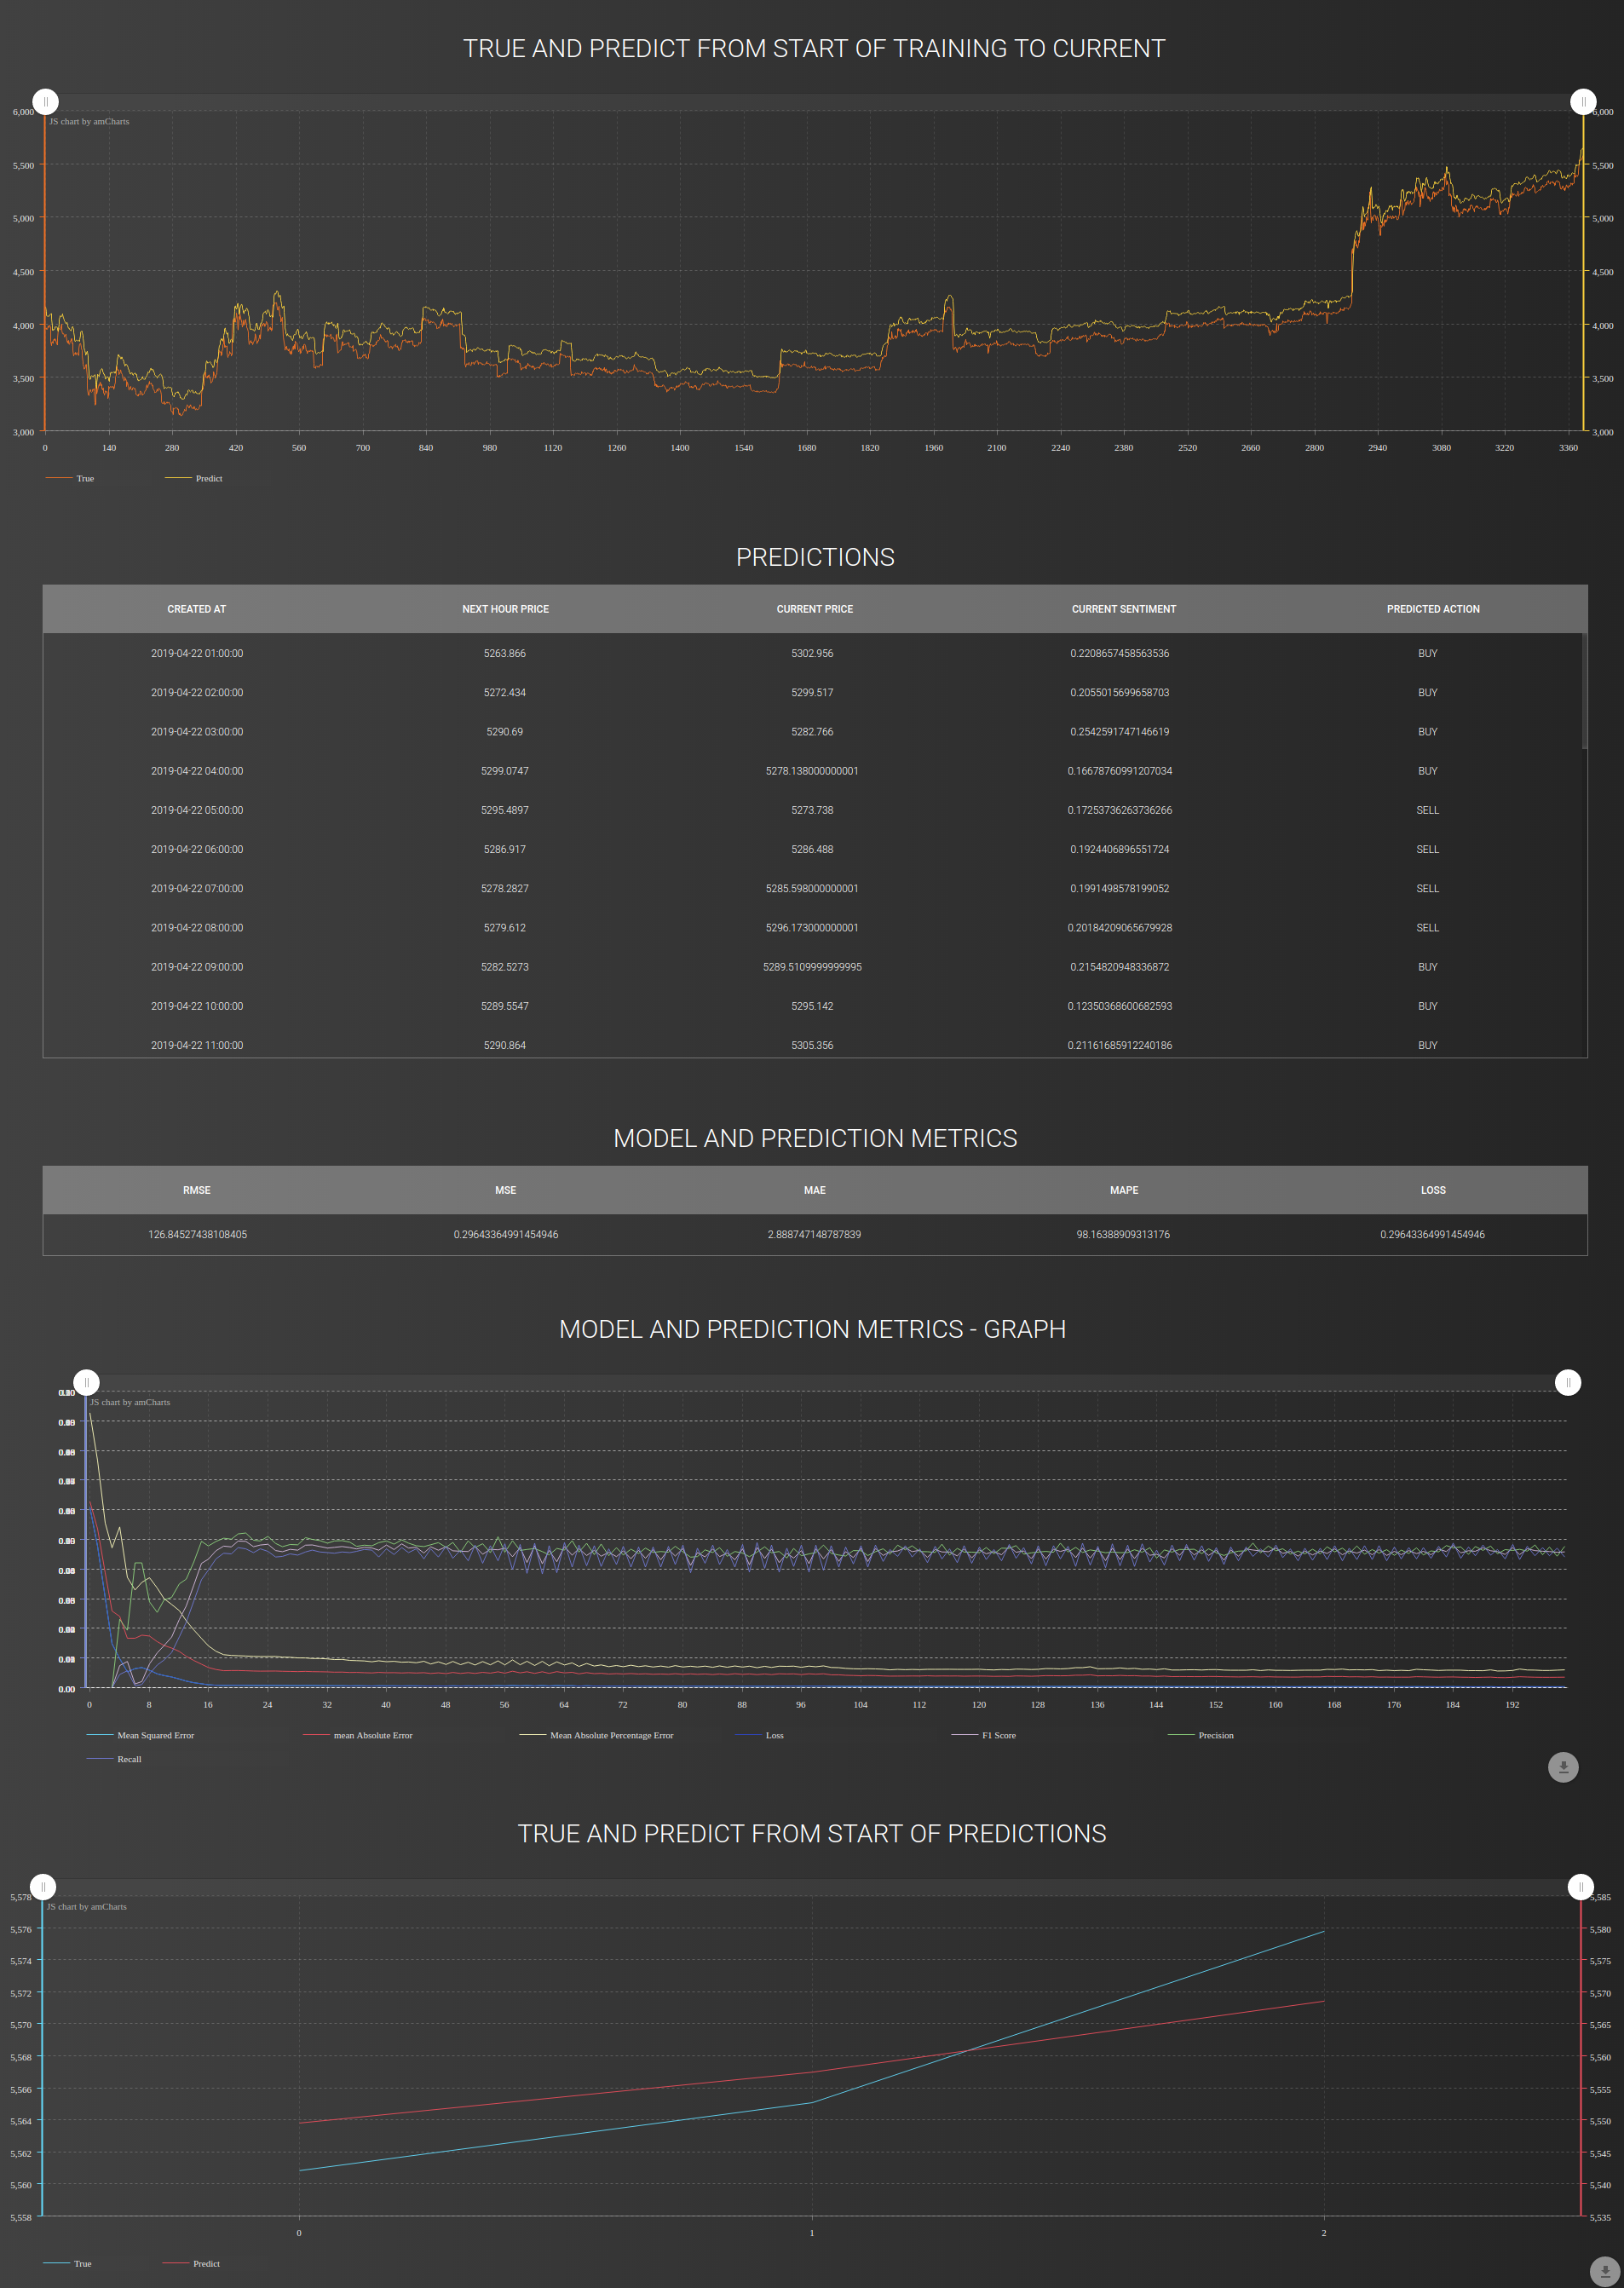
\includegraphics[width=14cm,height=19cm]{images/final_interface.png}
			\begin{center}
				\textit{Figure 12: Final Interface - \url{cryptosky.me} and \url{nosent.cryptosky.me}}
			\end{center}
		\end{figure}
		
	\newpage
	
	\section{Testing Metrics and Accuracy}
	This section discusses the performance metrics used to validate the network, any additional validation step during training, speed of execution of the two networks, and outlines what these mean regarding the performance of the network. 
	
	Due to that the project is primarily an investigation of the use of discussed tools on how these would be used for forecasting the price of the next hour of Bitcoin, based on both historic and live price, and sentiment data, testing is focused around the accuracy of the predicted hourly values and the model generated by the LSTM network. A discussion of the accuracy of the predicted values is discussed in the 'Discussion of Results' section along with comparing both models - with and without sentiment embedded to fulfil the problem statement.
	
	\subsection{Integration Testing}
	Integration testing occurred throughout the development of this system, the goal of this type of testing is the ensure that each of the functions within the system was working with previous functions that it either uses or provides functionality too and to conform to an agile methodology when possible.
	If and when a function was completed, prior to moving on to the development of another, the function was tested with real and fake data - depending on the functionality the function performed. This was to ensure that the function was either being access or used other functions correctly.
	
	An example of when such testing occurred, though not documented, between components is that of the \textit{FilterSpam} class in the \textit{tweet\_collector} script. This was a significant class to test the operation of and was due to both the multiple calling of functions within the class from throughout the \textit{tweet\_collector} script and from the functions of the class to individual functions in the \textit{spam\_filter} script. For a precise example, using \textit{Listing 9} and function \textit{testTweet}, this function is only ever called upon receiving data from the Tweepy streamer (\textit{Listing 4}), however, this function calls two other functions of \textit{processTweets} (\textit{Listing 8}) and \textit{classify} (\textit{Listing 11}) from the \textit{spam\_filter} script (detailed in the implementation section). Not only do each of these functions need to be tested that the correct data is being processed and returned, but the entire function is reliant on the classifier being already trained for classification which is handled by the function in the class, whom of which also call other functions from the \textit{spam\_filter} script (\textit{Listing 10}).
	
	This example was one of the most complex classes and set of functions to test as there was a lot of jumping back and forth and sequencing needed to ensure that the classifier was trained correctly and that streamed tweets are classified correctly. Similar testing occurred with all other functions and classes of the system at each stage of development.
	
	\subsection{Accuracy of Model \& Results}
	Due to the type of neural network used and its use case, suitable regression metrics were chosen to identify the accuracy of the model used for forecasting the next hour price of Bitcoin. As mentiod in the implementation section, subsection \textit{Training and Testing Model} the metrics used are as follows:
	
	\begin{center}
		\begin{tabular}{c|c|c|c|c}
			\textbf{RMSE} & \textbf{MSE} & \textbf{MAE} & \textbf{MAPE} & \textbf{Loss}\\
			\hline
			\multirow{1}{*}{} 100 $\pm$ 20 & 0.3 $\pm$ 0.1 & 3.0 $\pm$ 0.5 & 10\% $\pm$ 5\% & 0.3 $\pm$ 0.1 \\
		\end{tabular}
	\newline
	
			Per execution of the neural network - \textbf{with} sentiment embedded
	\end{center}

\begin{center}
	\begin{tabular}{c|c|c|c|c}
		\textbf{RMSE} & \textbf{MSE} & \textbf{MAE} & \textbf{MAPE} & \textbf{Loss}\\
		\hline
		\multirow{1}{*}{} 100 $\pm$ 25 & 0.3 $\pm$ 0.15 & 3.0 $\pm$ 0.5 & 10\% $\pm$ 6\% & 0.3 $\pm$ 0.15 \\
	\end{tabular}
	\newline
	
	Per execution of the neural network - \textbf{without} sentiment embedded
\end{center}

	\subsubsection{Results Discussion}

	The results, although exceptionally close for each network (with and without sentiment embedded), averaged over 50 runs of each network show that the model with sentiment embedded generally performs better than the model without sentiment used in predictions. The model with sentiment embedded has an average RMSE of 100 give or take 20 per each run which shows that on average the predictions are closer to the regression line than the model without sentiment. Additionally, the mean absolute percentage error discrepancy is less for the model with sentiment embedded than the model without. This, however, does not provide a clear distinction between the two models that is needed to justify what is outlined in the problem statement.
	
	A clearer distinction between the performance of the two models is when the metics are showing the two model performing almost as accurate, as in the RMSE of both has been 105 and 106, the closest it has been on the 50 runs during testing. This also saw the mean absolute percentage error have only 0.2\% difference between the two models. Unfortunatly, the difference between the two models can only be seen when a portion of predictions are made. The models were left to run for 48 hours each which returned 48 predictions each of which could be compared to the next hour price.
	
	\begin{center}
		\begin{tabular}{c|c|c|c}
			\textbf{Created at} & \textbf{Prediction} & \textbf{Current Price} & \textbf{Current Sentiment}\\
			\hline
			\multirow{1}{*}{} 2019-04-22 6pm & 5308.333 & 5318.4119 & 0.24312407 \\
			\multirow{1}{*}{} 2019-04-22 7pm & 5309.2754 & 5373.438 & 0.21355466 \\
			\multirow{1}{*}{} 2019-04-22 8pm & 5310.557 & 5413.161 & 0.28671014 \\
			\multirow{1}{*}{} 2019-04-22 9pm & 5317.3716 & 5375.6269 & 0.22499429\\
			\multirow{1}{*}{} 2019-04-22 10pm & 5337.3213 & 5373.607 & 0.25170501 \\
			\multirow{1}{*}{} 2019-04-22 11pm & 5370.356 & 5386.581 & 0.26898607\\
			\multirow{1}{*}{} 2019-04-23 12am & 5386.6113 & 5392.774 & 0.22517575\\
			\multirow{1}{*}{} 2019-04-23 1am & 5386.9487 & 5387.8319 & 0.27451984\\
			\multirow{1}{*}{} 2019-04-23 2am & 5379.05 & 5380.0669 & 0.23613823\\
			\multirow{1}{*}{} 2019-04-23 3am & 5384.681 & 5386.57 & 0.24832858\\
			\multirow{1}{*}{} 2019-04-23 4am & 5388.9434 & 5399.268 & 0.25803705\\
			\multirow{1}{*}{} 2019-04-23 5am & 5386.557 & 5429.906 &  0.25804942\\
			\multirow{1}{*}{} 2019-04-23 6am & 5385.1934 & 5510.472 &  0.25270584\\
			\multirow{1}{*}{} 2019-04-23 7am & 5389.97 & 5533.843 &  0.34432973\\
			\multirow{1}{*}{} 2019-04-23 8am & 5406.9917 & 5531.68 &  0.34782233\\
			\multirow{1}{*}{} 2019-04-23 9am & 5449.7676 & 5534.522 &  0.27746379\\
		\end{tabular}
		\newline
		
		15 records of predictions - \textbf{with} sentiment embedded
	\end{center}

\begin{center}
	\begin{tabular}{c|c|c}
		\textbf{Created at} & \textbf{Prediction} & \textbf{Current Price}\\
		\hline
		\multirow{1}{*}{} 2019-04-22 6pm & 5373.431 & 5318.4119 \\
		\multirow{1}{*}{} 2019-04-22 7pm & 5381.814 & 5373.438 \\
		\multirow{1}{*}{} 2019-04-22 8pm & 5381.952 & 5413.161 \\
		\multirow{1}{*}{} 2019-04-22 9pm & 5388.013 & 5375.6269 \\
		\multirow{1}{*}{} 2019-04-22 10pm & 5410 & 5373.607 \\
		\multirow{1}{*}{} 2019-04-22 11pm & 5442.346 & 5386.581 \\
		\multirow{1}{*}{} 2019-04-23 12am & 5457.733 & 5392.774 \\
		\multirow{1}{*}{} 2019-04-23 1am & 5460.422 & 5387.8319 \\
		\multirow{1}{*}{} 2019-04-23 2am & 5451.898 & 5380.0669 \\
		\multirow{1}{*}{} 2019-04-23 3am & 5457.16 & 5386.57 \\
		\multirow{1}{*}{} 2019-04-23 4am & 5461.436 & 5399.268 \\
		\multirow{1}{*}{} 2019-04-23 5am & 5459.212 & 5429.906 \\
		\multirow{1}{*}{} 2019-04-23 6am & 5457.895 & 5510.472 \\
		\multirow{1}{*}{} 2019-04-23 7am & 5461.916 & 5533.843 \\
		\multirow{1}{*}{} 2019-04-23 8am & 5479.55 & 5531.68 \\
		\multirow{1}{*}{} 2019-04-23 9am & 5523.663 & 5534.522 \\
	\end{tabular}
	\newline
	
	15 records of predictions - \textbf{without} sentiment embedded
\end{center}

	\begin{figure}[hbt!]
		\centering
		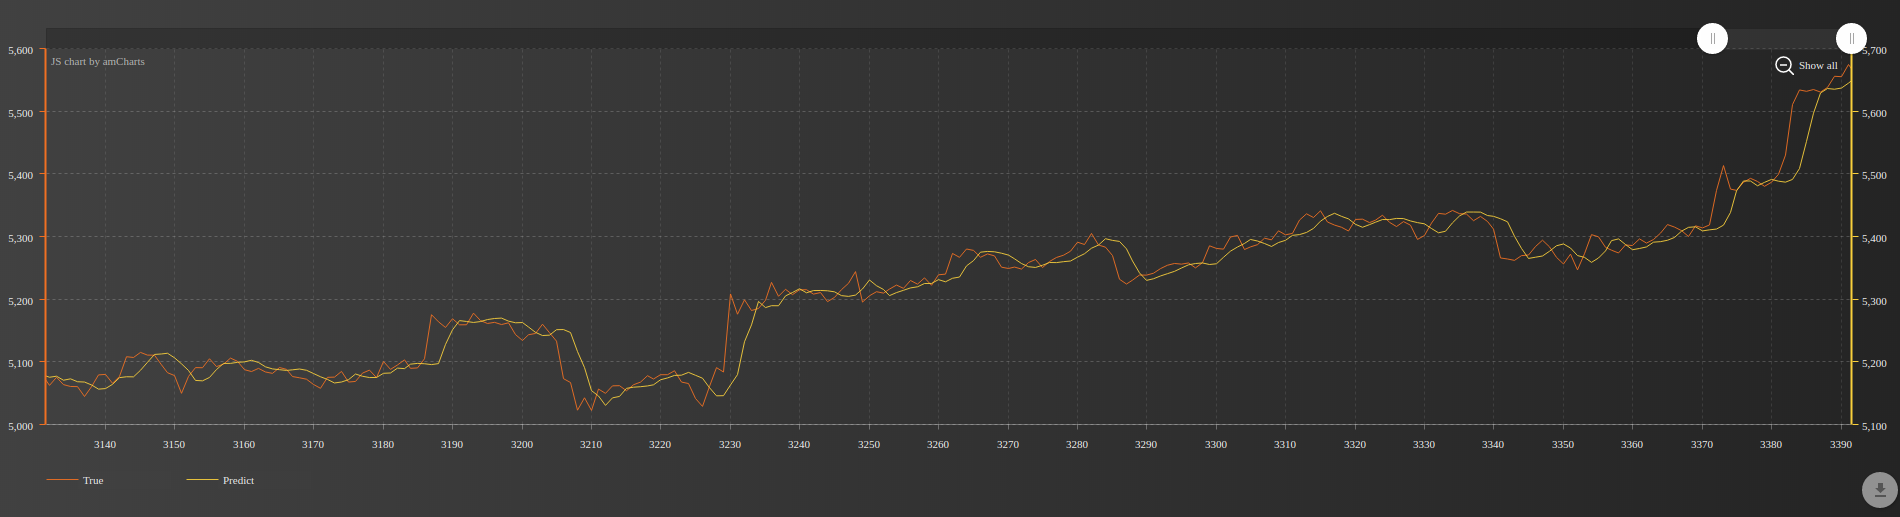
\includegraphics[width=16cm,height=6cm]{images/with_sentiment.png}
		\begin{center}
			\textit{Figure 13: \url{cryptosky.me} - model \textbf{with} sentiment embedded}
		\end{center}
	\end{figure}

\begin{figure}[hbt!]
	\centering
	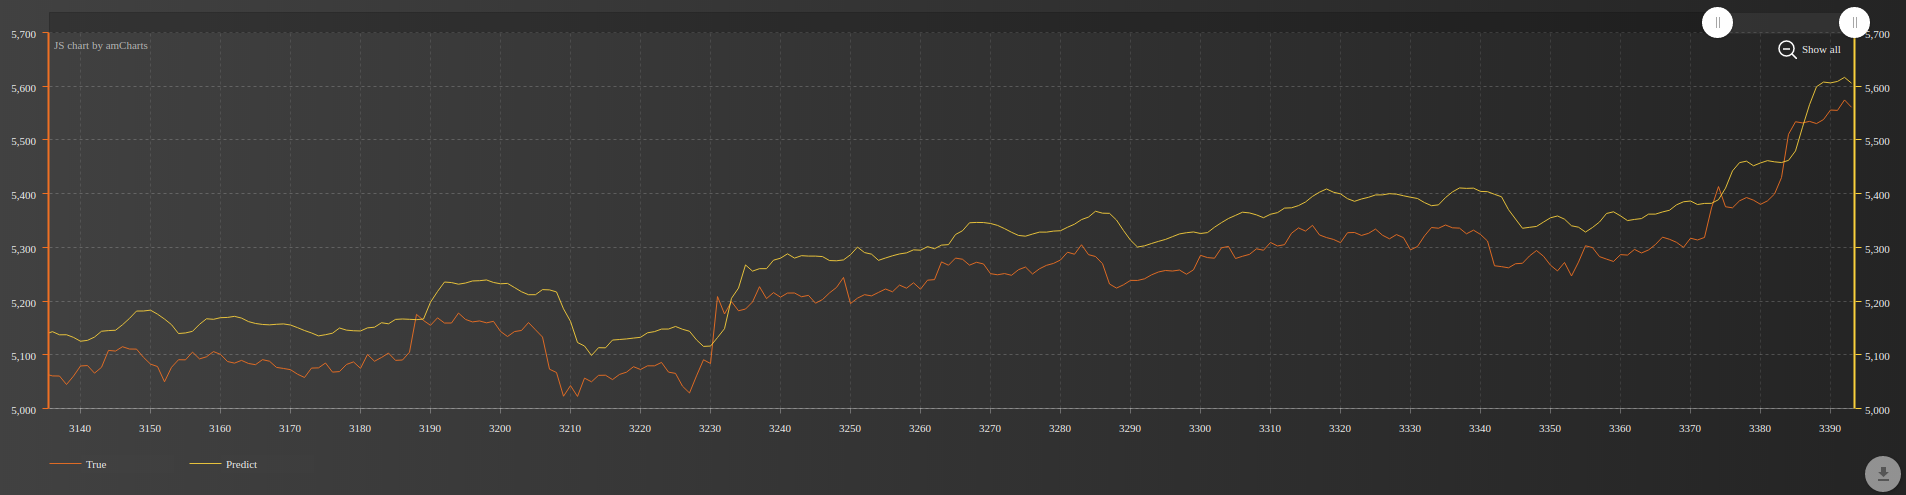
\includegraphics[width=16cm,height=6cm]{images/without_sentiment.png}
	\begin{center}
		\textit{Figure 14: \url{nosent.cryptosky.me} - model \textbf{without} sentiment embedded}
	\end{center}
\end{figure}

\newpage
	
	On visual inspection, after both models had made 48 predictions, \textit{See above tables} showing 10 records as an example, it can be seen that the model with the sentiment embedded both follows the current price more closely and is not as conservative in its predictions as the model without sentiment. 
	How conservative the model without sentiment embedded is can be seen in the five values between, 1 am to 5 am, where it attempts to correct itself to the actual value but slow to do so, then predicts a higher price for the next hour. At a point, the predicted value somewhat resembles that of the actual price but only due to the exact price rising substantially.
	This model through the data shown shows that it takes much longer to change the prediction to the actual real value of the next hour compared to the model with the embedded sentiment. 
	Also, neither model handles spikes in prices very well which is more noticeable with the model with sentiment as it follows the exact price more closely.
	
	Another factor that can be identified by the results shown above is that the model with the sentiment embedded in with the price data doesn't react adequately for when the sentiment spikes - regardless of a price spike. This could suggest that the data has not been predicted using enough data of both price and sentiment, due to only training on the last five live prices and sentiment and not 1000 samples to match the batch size the model was trained on during model creation. An improvement to the model could be made during predictions of the next hour price where it continuously predicts on the data available until it has 1000 records, then only predicts using the last 1000 records of live data. At this point, 1000 hours into predictions, said predictions might become more accurate than what is presented for evaluation at the time of writing due to matching the training batch sample size of the trained model of the network.
	
	Another result that can be drawn from the data presented, separate from the models' performance, is that of how sentiment affects the following hours' price. It can be seen in a number of the records presented that the sentiment occasionally spikes, at 1 am spikes to \textit{0.27451984} from the previous hour of \textit{0.22517575}, and the spike is not represented in the following hours' price. This also occurs on a previous hour at 8 pm which saw a spike of sentiment, a \textit{0.07405548} difference from the previous hour but saw the price drop almost \$40. This could indicate that the sentiment of the hours does not directly affect the next hours' price but affects it over possibly several hours, and also shows that there is not a direct correlation in sentiment spikes to price spikes.
	
	\subsubsection{Execution Speeds}
	Each of the models are trained and validated using both generated training and testing dataset over 200 epochs and a batch size of 1000 on 11000 records total of data, within minutes. The network with sentiment embedded take marginly longer to create the prediction model.
	
	\begin{center}
		\begin{tabular}{c|c}
			\textbf{Network} & \textbf{Speed} \\
			\hline
			\multirow{1}{*}{} With Sentiment & 3:15 $\pm$ 0:20 secs\\
			\multirow{1}{*}{} Without Sentiment & 2:50 $\pm$ 0:20 secs\\
			
		\end{tabular}
		\newline
		
		Speed of executions of each network, averaged over the 50 testing runs
	\end{center}
	
	\newpage
	
	\section{Discussion: Contribution and Reflection}
	The testing performed and the results obtained show significant difference using sentiment alongside price can have on the forecasting of the next hours' price of Bitcoin, visually shown in \textit{figures 13 \& 14}. Results have also identified that both models do not handle spikes in both sentiment or price adequately, as seen in \textit{figures 13 \& 14} it usually takes another hour for the spike to be reflected in the predictions, longer so for the model without sentiment embedded. Also stated in the discussion of the results, it can be seen that the sentiment of the hour does not directly or immediately affect the next hours' actual price, even when there is a spike or drop in sentiment or price. As stated this could suggest that sentiment affects the price over a broader time range such as a few hours, and also shows that there is no direct correlation between, in the data presented, sentiment spikes to price spikes.
	
	With testing and results discussed it is important to discuss some of the general issues that occurred during the development that contribute to the results shown and identifying correlations to solve the problem statement. 
	
	One issue is that of deployment and the need to have the system continuously running to make hourly predictions and to satisfy the problem statement of providing a system to aid in investor decision making of the market. Additionally, the system needs to continuously run to meet the batch file size, which will aid in determining if predicting on 1000 records shows if predictions become more accurate on each iteration after 1000 records have been obtained, as mentioned and described in the discussion of the results section.
	The current solution that has been used to during development is to run the system for training purposes on a work laptop while the front-end is hosted on an external cloud server. On each hour a prediction is made a bash script watches the relevant files that contain predictions, performance metrics and correct over predicted values for graph plotting for changes, and is then SCP'd (Secure Connection Protocol) to the relative path on the cloud server for the front-end to access and display to the stakeholders.
	Due to the cost and computational power needed, and system not working when initially attempting to deploy it to the server, it was impractical to host it on an external server for the given time frame needed for completion of this project.
	A proper solution would see both systems deployed at a production level with both fully operational on the external server.
	
	Another issue, relating to the issue just described is that on system execution being halted. The issue is that during the period in which the system is not running live prices and sentiment are not being collected, ignoring that predictions are not made. When the system is brought back online it will be missing the now 'historical' data for that given period when it was not running and collecting data; thus this data has to be manually entered. Due to the system not being deployed in 'production' and was ran from a personal laptop this issue frequently occurred, which would be mitigated if it was deployed to an external server. If the system were to crash on a production server, there are several try-catch statements throughout the system that will restart the processes if this issue occurs.
	
	\subsection{Limitations}
	The limitations of the system can be quite clear, as described extensively already with both models performances. However, it is important to identify which points in the technical specifications the final developed system did not meet.
	
	Looking back at the technical specification laid out at the start of this project, there is only one point that this system does not meet. It is that of 'both prediction system and interface, should be deployed to a server due to the need to be constantly running'. As already discussed in the discussion section prior to this section, it was both unfeasible for several factors and to get fully operational. This was due to the difference in execution speeds of the laptop used compared to the server intended for deployment, timings in which the model was planned to train on did not match or work on the deployment server thus data collection and predictions made became increasingly later until an hour was left out. Additionally, a limitation that was presented was that of the server intended for deployment was in UTC and not on a GMT timezone in which the development laptop was on which further affected the timings of forecasting and system execution. 
	
	Additionally, limitations would be identified if future improvements were to be implemented in the system. Although these improvements are outlined below in the \textit{future improvements} section, one such one that would be suitable to discuss initially as an example would be that of comparing how tailoring the VADER lexicon with domain specific language. Language such as \textit{bullish}, \textit{bearish} and \textit{shorting} terms with identified and relevant weighted sentiment values would have on the outcome of the polarity classification of the VADER analyser, and how this also could more significantly affect the next hour forecasting of Bitcoin price. Due to the VADER sentiment analyser lexicon being open-source these additions would be reasonably easy to implement, the real task, however, would be on how to identify the suitable weighted sentiment value for the specific words added, which in itself could be an entirely new project.
	
	Lastly, a limitation that could be identified and is also discussed in the results section above is that of the performance metrics not showing a clear distinction between the two network models. This limitation could be overcome by using more suitable explanative metrics, rather than relying on a more visual inspection, such as: 
	\begin{itemize}
		\item Adjusted $R^2$ statistic - Shows how well the selected independant variables of the model explain the variability of the dependant variables, and shows how well the terms fit a regression line \cite{RMSEMAE}. 
		\item Mean Bias Error (MBE) - Is the Mean Absolute Error (MAE), but is calculated if the absolute value isn't taken (the signs of the errors are not removed) the MAE becomes the mean biased error. The MBE is intended to measure the average model bias and can convey more useful information that the MAE, but should be interpreted with caution due to the positive and negative error cancelling out. \cite{MBE}
	\end{itemize}
	By calculating these metrics could aid in distinguishing a correlation between the models based on metrics rather than on visual analysis.
	
	
	\subsection{Reflection}
	Developing this project has opened my eyes up to the development of exciting topics that have been used to make the solution of this project real. It has taught me the basics of natural language pre-processing the steps involved to form the data correctly for classification, both how this would be used for a spam classification algorithm like the one implemented and for a traditional machine learning based sentiment analyser. On top of this, it has allowed me to discover other methods for sentiment analysis such as lexicon-based approaches such as VADER and how customisable to a topic domain they are when the lexicon is either altered or added to - along with how the weighted sentiments are formed (based on knowledge from the VADER paper \cite{VADERPaper}). 
	
	This project has taught me the basics of how both neural networks, recurrent neural networks and LSTM recurrent neural networks function and how they compare to each other in terms of performance for a particular task of time-series forecasting and their suitability for this task - quantified as knowledge from relevant sources used within the literature review. Known issues of each network such as exploding gradients and how an LSTM network overcomes these standard RNN issues. An in-depth understanding of the low-level functionality of an LSTM network, optimisers available - use, suitability and operation, regularisation techniques and dropout for minimising overfitting and underfitting of the network with the training datasets.
	
	It has taught me how the classical (multinomial) naive Bayes probability model can be used for classification for spam or ham (wanted) data, and how the underlying maths and algorithm works - due to hand-coding the algorithm from scratch. Through the use of both the Bag Of Words algorithm for term-frequency identification: how it builds upon the base probability model of the Bayes algorithm. How TF-IDF (Term Frequency-Inverse Document Frequency) further builds upon this to both identify the amount of occurrence of words in a given text by assigning a weight, but also how it uses this to identify commonly used words that are of no relevance to classification. Further how the Addictive Smoothing method aids in dealing with words that have not been identified during training, due to not being initially presented in the training data.
	
	Development of this project has given me a further understanding of time management and priorities, in the sense of what needs to focused on during development prior to other features being coded or implemented. An excellent example of where priorities had changed can be seen from the original PID form, \textit{Appendix B}, in which the solution to this project changed from focusing on the front-end application to focusing on the back-end system. This was due to a few factors that have already been identified in the Solution approach section. Where both stakeholders, I the developer and the supervisor of the project concluded that the creation of a front-end application, with a basic back-end for predictions, would not be a satisfactory solution, and more focus should be invested into the price predictions of Bitcoin. Another point where time management had to be considered was when implementing the Naive Bayes Classifier for spam filtering. Time management was not considered during its development and saw the feature go out-of-scope for what was initially wanted - the initial idea was to use the scikit-learns in-built Multinomial Naive Bayes classifier for spam classification. However, tutorials were found on top of the papers used for describing the algorithm during the literature review, which further described how to implement such an algorithm from scratch. Thus this was undertaken and leading to arguably time wasted coded the classification model rather than spending more time on coding the neural network. Arguably in a sense, as detailed in the previous paragraph, it taught me a great deal of how the algorithm works, and it's limitations.
	
	Furthermore, it has allowed me to form a better knowledge base and understanding of the Python language and data mining techniques used for the languages, to manipulate and used data for a required purpose, and has taught me relevant useful performance metrics for identifying the performance of a neural network and what the results of the metrics represent.
	
	Lastly, if I were to conduct this project again, I would create a new lexicon that is explicitly tailored to the type of language used in the stock market as it has a unique language, and how suitable sentiment weights would be assigned to the new words. I would also adjust and alter both the batch size and epoch amount to identify how this affects the training and accuracy of predictions for both networks - with and without sentiment. I would also create a more refined and developed user interface for production level, which will more appropriately satisfy the problem of the public not having a system available to aid in investment decision making. The current interface, although providing relevant and useful information which would still be the information displayed to the stakeholders and users, the interface could be significantly improved to meet a production level solution. More arguably I would build upon what this project has become and implement the future improvements laid out in the \textit{fucute improvements} section below. Most notably a future improvement that would be implemented would be that of additional performance metrics such as $R^2$ statistic and Mean Bias error along with K-fold Cross-Validation (which was not implemented due to time constraints and not knowing how to implement this for continuous data). This will be used to justify further both the performance of the two networks with validation of the model and to accurately identify a correlation between how sentiment affect the price of bitcoin and the accuracy of the network with it embedded, rather than relying on visual inspected as used for the majority of the results discussion.
	
	\section{Social, Legal and Ethical Issues}
	During the creation of the Project Initiation Document, with the intended solution, no foreseeable Social, Legal or Ethical Issues were identified. As the concept and solution changed considerably both before proper development and also during development, no other Social, Legal or Ethical Issues presented themselves. There was however a developer agreement policy that was required to be agreed with prior being able to access the Twitter API, for both historical tweets and with use with the Tweepy Python package. This document outlined various limitations of the use of the API such as rate limits and security personal security of generated API keys, but nothing significant that affected the development of the project apart from the mentioned section of reverse engineering the Twitter API, in which this project had not set out to do. As tweets posted on Twitter are public and free to access by anyone there are no personal information issues that could be presented; thus this agreement was no a Social, Legal or Ethical issue. \textit{Twitter API - Developer Agreement and Policy} \cite{TwitterTerms}
	
	\newpage
	
	\section{Conclusion and Future Improvements}
		\subsection{Conclusion}
		As stated, the projects focus and solution changed considerably from the original Project Initiation Document which stated in section 2.2 of the document that, the main objective was to "produce a thin web client that provides a dashboard, that provides tangible and useful information to users such as; current price" - \textit{of a cryptocurrency} - "exchange rate, network hashrates and historical price data". "It will also display statistics about sentiment analysis conducted on social media about the currency" with "graphical predictions on what the price may be, in a given time". As from the extracts, the initial objectives of the project were broad and also vague. As this suggests that the focus of the project will be that of creating a thin client dashboard which was no longer the focus of the project, and \textit{"about the cryptocurrency"}, indicating sentiment analysis and price predictions would be conducted on multiple currencies which were an extremely board estimations of workload. It does, however, show that the initial thought process of performing sentiment analysis and price predictions occurred during initial stages of this project, but ultimately change through development to focus on how said sentiment of a cryptocurrency, Bitcoin, extracted from social media could be used in aiding in the prediction of future price.
		
		As for reference to the projects problem statement and solution approach, "This project will focus on the investigation of these technologies and tools", (sentiment analysers, machine learning algorithms and neural networks), "to justify whether it is feasible to predict the price of BTC based on historical price and the sentiment gathered from Twitter". The solution outlined in the solution approach stated that the solution is "to create a system mainly consisting of; a frontend application that will display plotted; predicted and true, performance metric data to the user as a clear and concise form". A back-end prediction system of "various subsystems responsible for data collection, filtering, data pre-processing, sentiment analysis, network training, validation and training, and future price predictions".
		
		The end result followed suitably with would was outlined in both the problem statement and solution approach, and meet all but one point in the technical specification previously discussed in the reflection - where there were issues with deploying the back-end responsible for price forecasting to the external cloud server and getting it operational. A front-end application was also created, although basic, served its purpose of presenting the required data to users in a clear format. The back-end also suitably performed all the tasks set out for it such as; data collection from the Twitter API, sentiment analysis using VADER, and predicting the next hour price of Bitcoin.
		
		The majority of the focus was invested into implementing the back-end prediction solution, although fully implemented as intended some time was wasted hand-coding from scratch the Naive Bayes classifier. This did provide valuable information on exactly how the algorithm worked, its limitations and how additional techniques and methods overcome these but was ultimately wasted time due to an already used Python package, Scikit-Learn, having multiple in-built Naive Bayes models to choose from. If used, would have reduced time coding which could have been used elsewhere on the project. For example during testing, to implement K-fold Cross-validation, the $R^2$ statistic or produce the Mean Bias Error, and in turn possibly aid in identifying a correlation from the metrics between the two models, with and without sentiment, rather than relying on the metrics used which did not show much and visual inspection of prediction results.
		
		To conclude, the system that has been developed to meet the requirements set out for this project has been developed to the highest possible standard in the time frame that was given for this project. Moreover, from the discussion of results, it can be believed that the system works well and predicts the next hour price of Bitcoin appropriately given the data provided. The user interface provides the necessary information, although not pretty, to the possible stakeholders in a clear and concise which is what was intended for the interface.
		
		
		\subsection{Future Improvements}
		
		
		
		
		
		as such comparing recurrent neural network models, implementation and the affect of regularisation techniques, use of different optimisers would have on the network, how use of ngrams could be used to improve language detection, comparing hand-coded naive bayes model to that of scikit-learns in built classifiers, alterations and additions to the VADER lexicon to tailor it with domain specific language and relevant weighted sentiment values
		
		Interesting what would a days prediction would show due to sentiment not directly affecting the next hour price
		
		Shifting the predicted data by and hour and sequencing over previous data - will also allow proper use of look-back windows
		
		Another could be to predict the hour of sentiment and create a threshold for it.
		
		Identify whether or not use of ngrams improved accuracy of spam classification
		
		Identify whether use lemmatisation would change how spam classification occured
		
		Look into use of other ngrams for use with language detection
		
		Compare Scikit-learns in-built naive bayes algorithms and other variations performance for spam filtering against hand-coded version
		
		Look into adding to the VADER lexicon for increasing performance and accuracy for topic domain of stock market language and what sentiment would be assigned to words
		
		IMPLEMENT AND IDENTIFY R2 stat and Mean Bias ERROR
		
		(R2 and mean bias error would be suitable metrics to show how conservative the model is and the difference between the predicted and true price it is) - never got to implement
		
		mean bias Error
		
		k-fold cross validation was attempted, but issues with continuous data
		How would this work what will it show or validate?
		
		How would changing epoch and batch size affect performance?
		
		Use a different charting system as the plotted lines seem to jump around and skew accuracy
	\newpage
	
	\nocite{*}
	\printbibliography
	
	\newpage
	\section{Appendices}
		\subsection{Appendix A - Project Initiation Document}
		Displayed on the following pages below.
		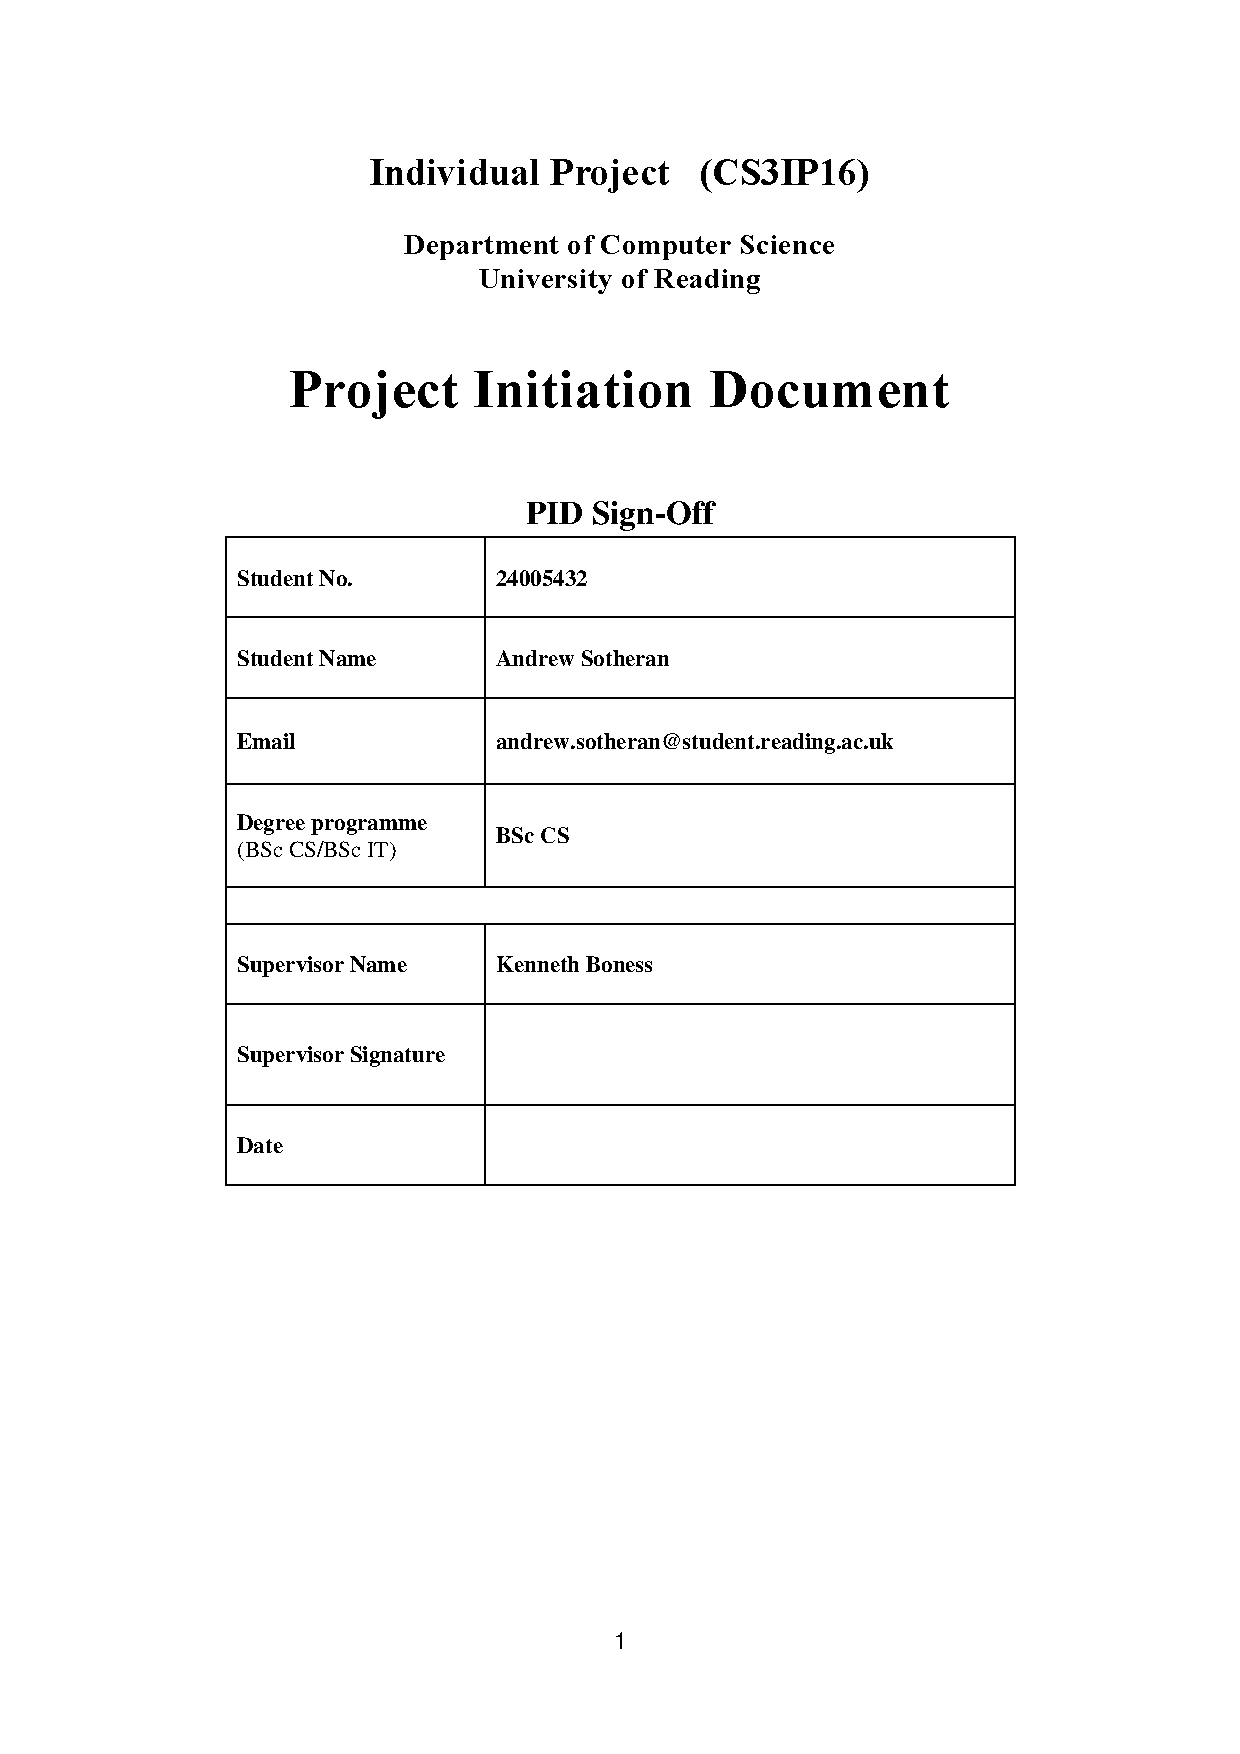
\includepdf[pages=-]{PID}
		
		\subsection{Appendix B - Log book}
		The log book for this project is a physical book and was handed to the School of Computer Science. Due to being a physical book, it cannot be inserted here.
	
\end{document}